\qrchapter{https://forgottenpillar.com/rsc/en-fp-chapter11}{The personality of God - by James S. White}


\qrchapter{https://forgottenpillar.com/rsc/es-fp-chapter11}{La personalidad de Dios - por James S. White}


In what follows, we will examine James White’s pamphlet titled “\textit{The Personality of God}”. When we read this article, we will see that James White continues where Brother Loughborough left off, and that he expands and deepens the understanding behind the first point of the \emcap{Fundamental Principles}.


En lo que sigue, examinaremos el panfleto de James White titulado “\textit{La personalidad de Dios}”. Cuando leamos este artículo, veremos que James White continúa donde el hermano Loughborough dejó, y que amplía y profundiza la comprensión detrás del primer punto de los \emcap{Principios Fundamentales}.


James White’s tract was printed multiple times, advertised 54 times, and reprinted twice in the Review and Herald publication. His view on the \emcap{personality of God} was well known and spread throughout Adventism. In this pamphlet, we will see clear criticism toward the ideas that Kellogg advocated in the Living Temple.


El tratado de James White se imprimió varias veces, se anunció 54 veces y se reimprimió dos veces en la publicación Review and Herald. Su punto de vista sobre la \emcap{personalidad de Dios} era bien conocido y se extendió por todo el adventismo. En este folleto, veremos una clara crítica hacia las ideas que Kellogg defendía en el Living Temple.


\begin{figure}[hp]
    \centering
    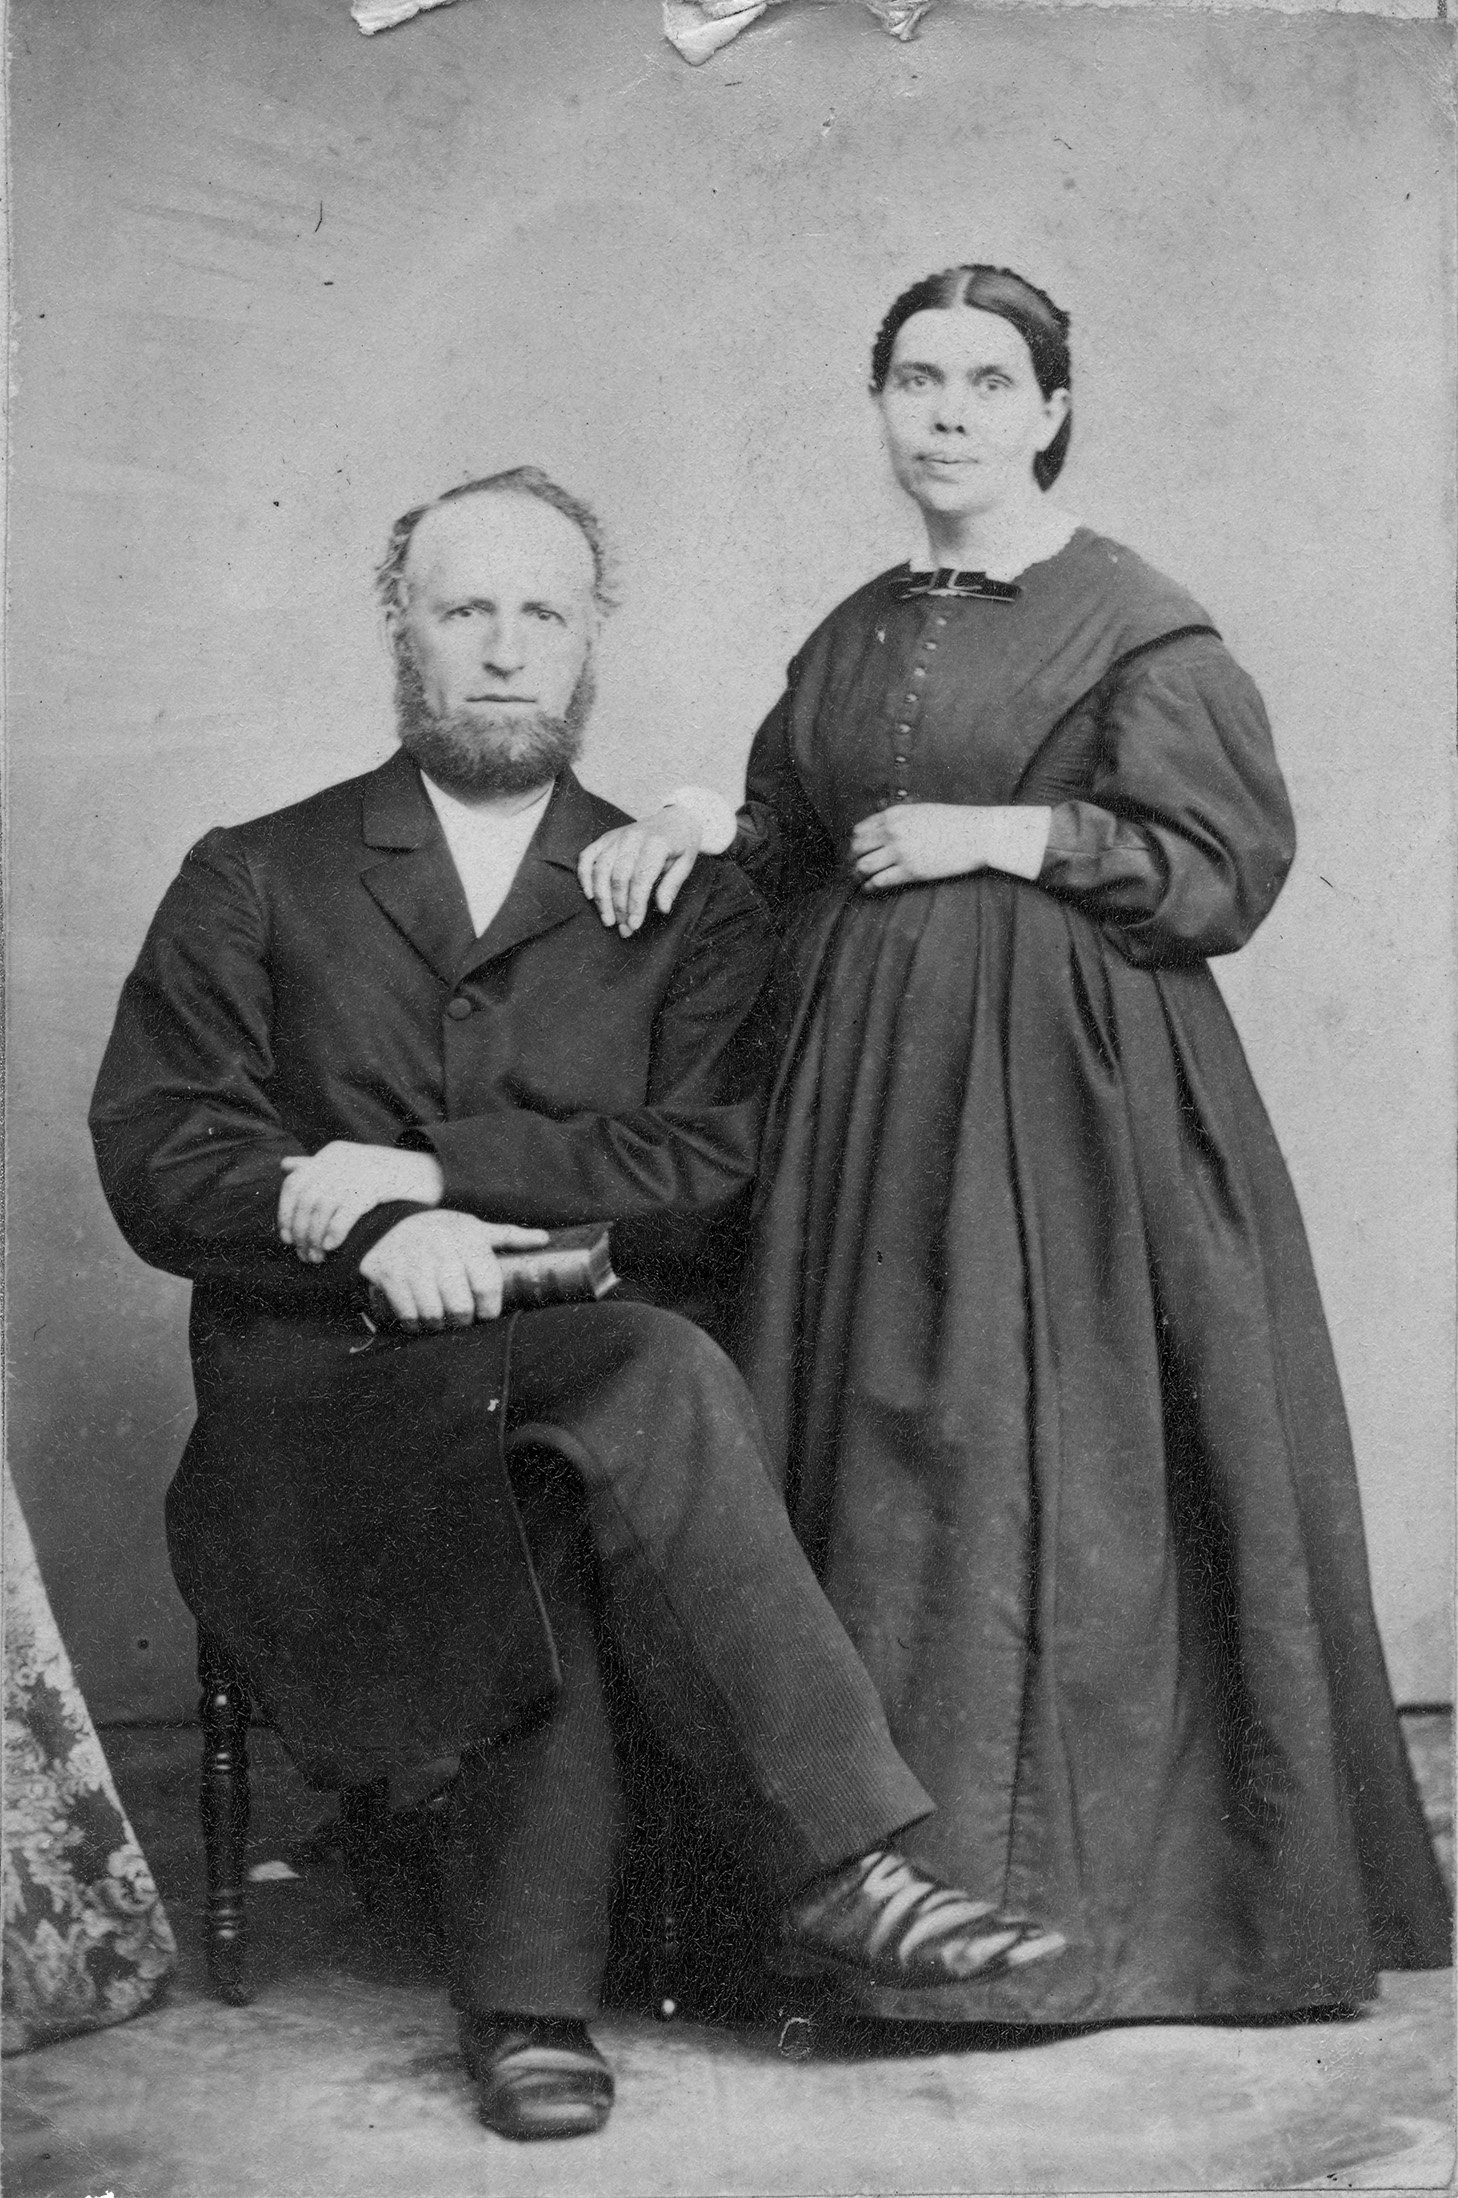
\includegraphics[width=1\linewidth]{images/james-and-ellen-white.jpg}
    \caption*{James Springer White (1821-1881) and Ellen White (1827-1915)}
    \label{fig:james-and-ellen-white}
\end{figure}


\begin{figure}[hp]
    \centering
    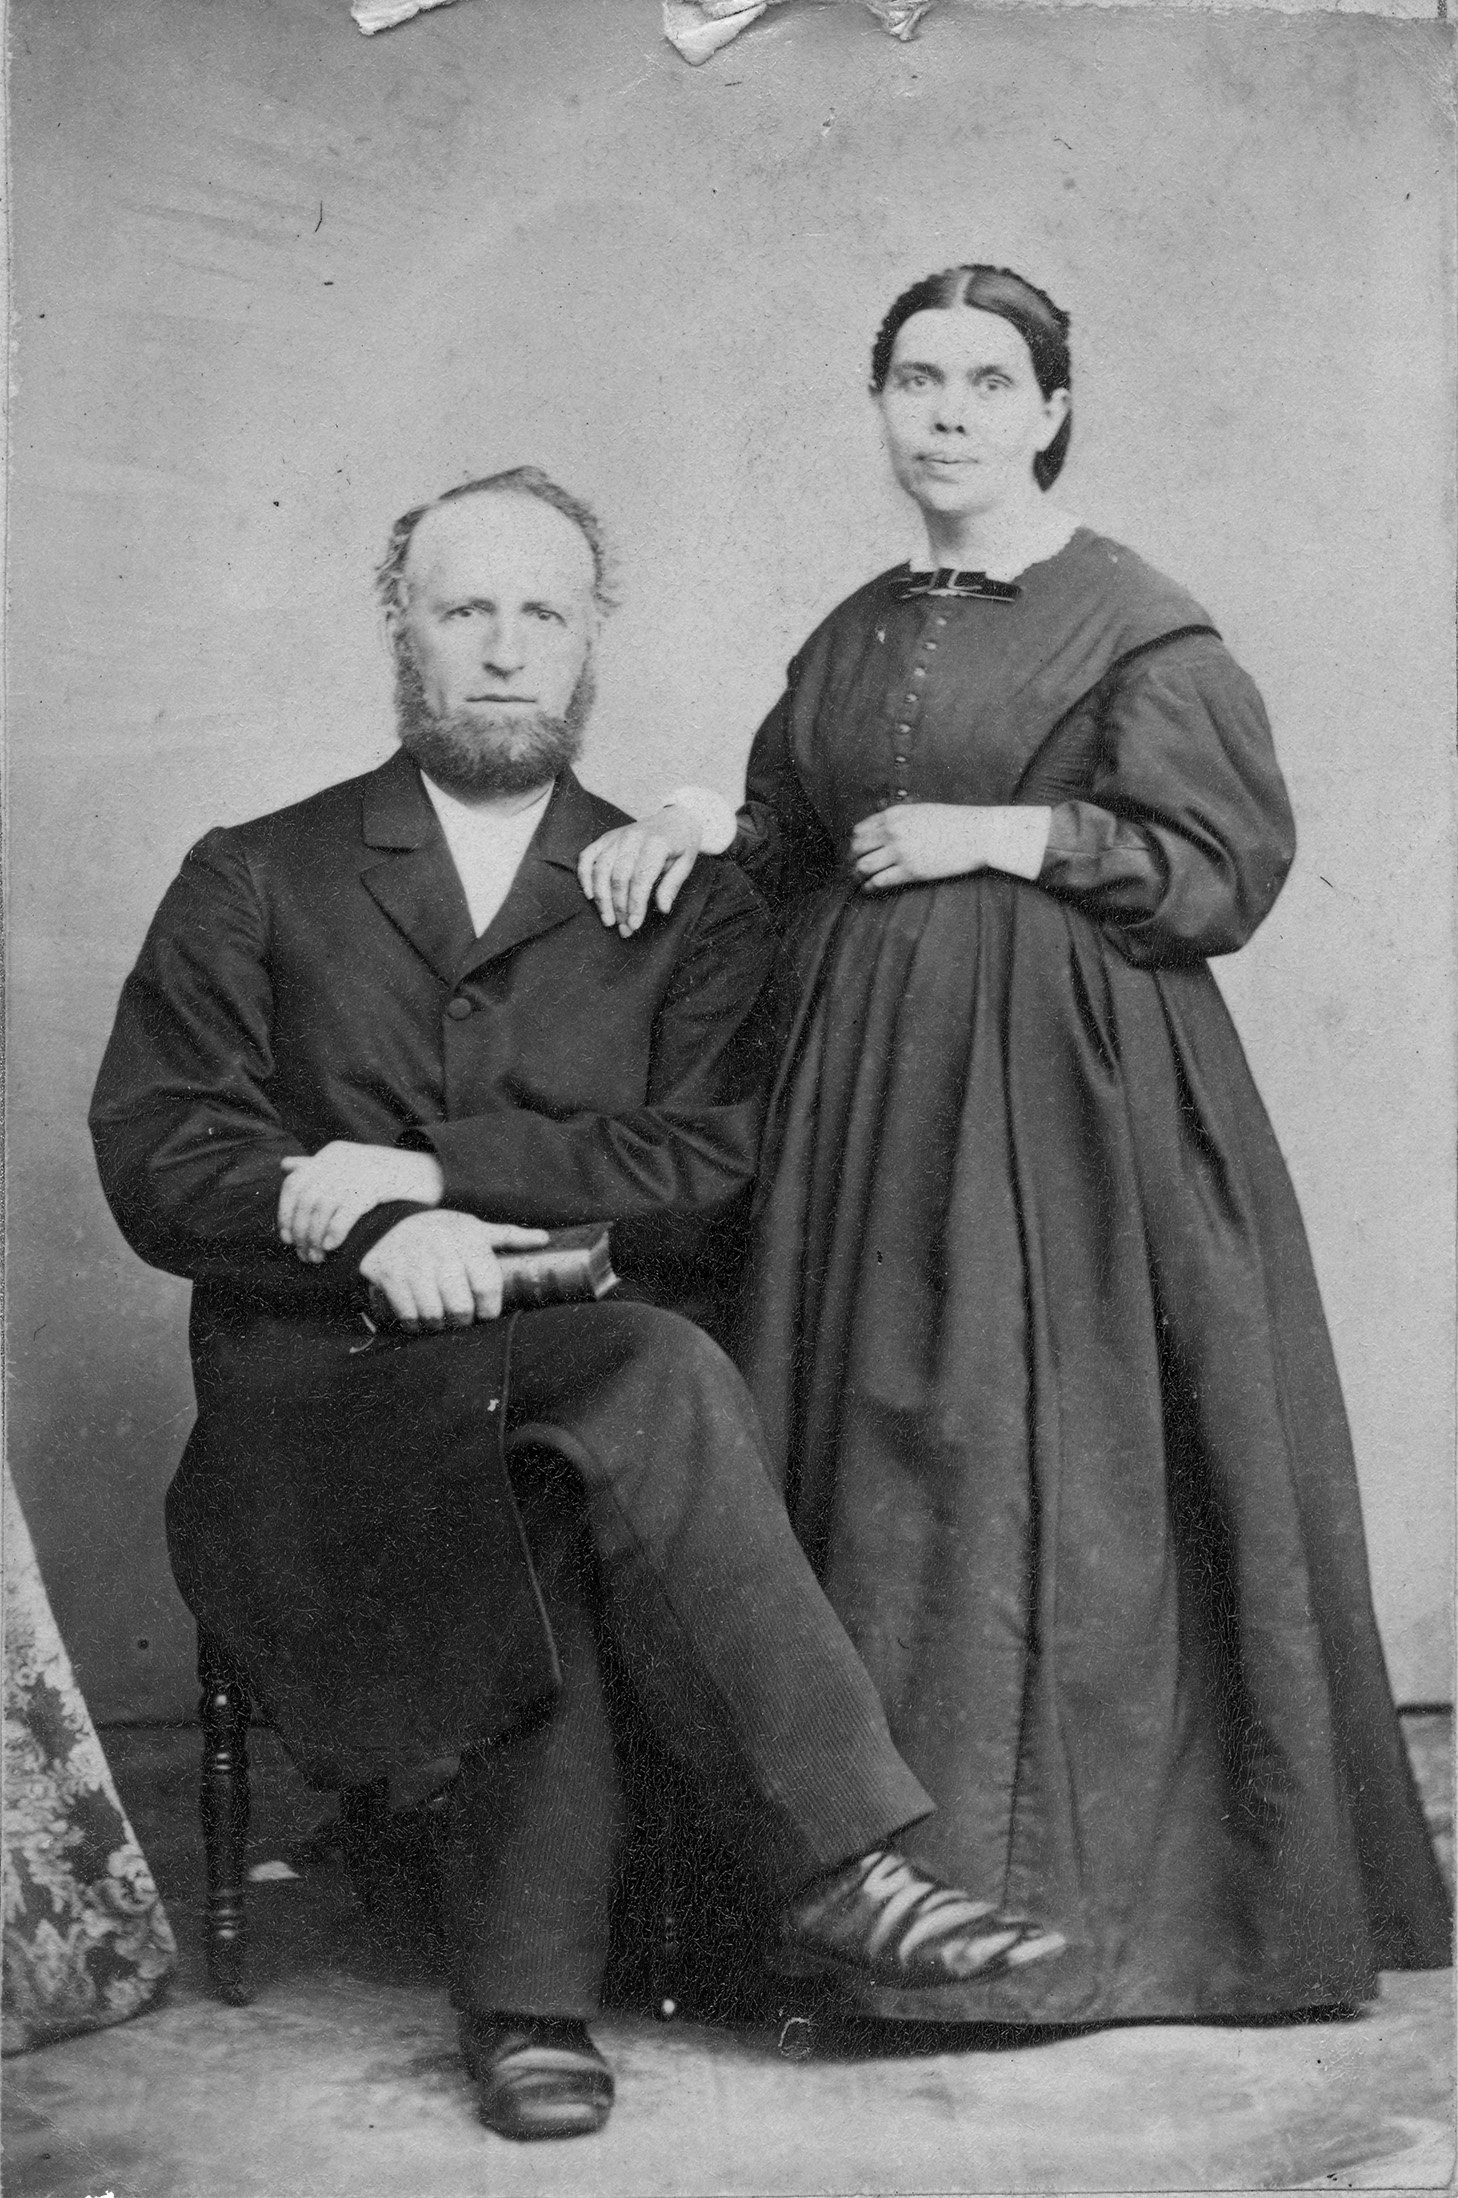
\includegraphics[width=1\linewidth]{images/james-and-ellen-white.jpg}
    \caption*{James Springer White (1821-1881) y Elena G. de White (1827-1915)}
    \label{fig:james-and-ellen-white}
\end{figure}


\othersQuote{\textbf{MAN was made in the image of God}. ‘And God said, Let us make man in our image, after our likeness.’ ‘So God created man in his own image, in the image of God created he him.’ Genesis 1:26, 27. See also chap. 9:6; 1 Corinthians 11:7. \textbf{Those who deny the personality of God, say that ‘image’ here does not mean \underline{physical form}, but moral image, and they make this the grand starting point to prove the immortality of all men}. The argument stands thus: First, man was made in God’s moral image. Second, God is an immortal being. Third, therefore all men are immortal. But this mode of reasoning would also prove man omnipotent, omniscient, and omnipresent, and thus clothe mortal man with all the attributes of the deity. Let us try it: First, man was made in God’s moral image. Second, God is omnipotent, omniscient, and omnipresent. Third, therefore, man is omnipotent, omniscient, and omnipresent. That which proves too much, proves nothing to the point, therefore the position that the image of God means his moral image, cannot be sustained. \textbf{As proof that God is a person, read his own words to Moses}: ‘And the Lord said, Behold there is a place by me, and thou shalt stand upon a rock; and it shall come to pass, while my glory passeth by, that I will put thee in a cleft of the rock, and will cover thee \textbf{with my hand} while \textbf{I pass by}. And I will take away \textbf{mine hand} and thou shalt \textbf{see my back parts}; \textbf{but my face shall not be seen}.’ Exodus 33:21-23. See also chap. 24:9-11. \textbf{Here God tells Moses that he shall \underline{see his form}}. \textbf{To say that God made it appear to Moses that he saw his form, when he has no form, is charging God with adding to falsehood a sort of juggling deception upon his servant Moses}.}[James S. White, PERGO 1.1; 1861][https://egwwritings.org/read?panels=p1471.3]


\othersQuote{\textbf{EL HOMBRE fue hecho a imagen de Dios}. ‘Y dijo Dios: Hagamos al hombre a nuestra imagen, conforme a nuestra semejanza’. ‘Y creó Dios al hombre a su imagen, a imagen de Dios lo creó’. Génesis 1:26, 27. Ver también cap. 9:6; 1 Corintios 11:7. \textbf{Los que niegan la personalidad de Dios, dicen que ‘imagen’ aquí no significa \underline{forma física}, sino imagen moral, y hacen de esto el gran punto de partida para probar la inmortalidad de todos los hombres}. El argumento es el siguiente: Primero, el hombre fue hecho a imagen moral de Dios. Segundo, Dios es un ser inmortal. Tercero, por lo tanto todos los hombres son inmortales. Pero este modo de razonamiento también probaría que el hombre es omnipotente, omnisciente y omnipresente, y así revestiría al hombre mortal con todos los atributos de la deidad. Intentémoslo: Primero, el hombre fue hecho a la imagen moral de Dios. Segundo, Dios es omnipotente, omnisciente y omnipresente. Tercero, por lo tanto, el hombre es omnipotente, omnisciente y omnipresente. Lo que prueba demasiado, no prueba nada al respecto, por lo que la posición de que la imagen de Dios significa su imagen moral, no puede sostenerse. \textbf{Como prueba de que Dios es una persona, léanse sus propias palabras a Moisés}: ‘Y dijo aún Jehová: He aquí un lugar junto a mí, y tú estarás sobre la peña; y cuando pase mi gloria, yo te pondré en una hendidura de la peña, y te cubriré \textbf{con mi mano} hasta que haya pasado. Después apartaré \textbf{mi mano}, y \textbf{verás mis espaldas}; \textbf{mas no se verá mi rostro}’. Éxodo 33:21-23. Véase también el capítulo 24:9-11. \textbf{Aquí Dios le dice a Moisés que \underline{verá su forma}}. \textbf{Decir que Dios le hizo parecer a Moisés que veía su forma, cuando no tiene forma, es acusar a Dios de añadir a la falsedad una especie de engaño malabarista sobre su siervo Moisés}.}[James S. White, PERGO 1.1; 1861][https://egwwritings.org/read?panels=p1471.3]


\othersQuoteNoGap{But the skeptic thinks he sees a contradiction between verse 11, which says that the Lord spake unto Moses face to face, and verse 20, which states that Moses could not see his face. But let Numbers 12:5-8 remove the difficulty. \textbf{‘And the Lord came down in the pillar of the cloud}, and stood in the door of the tabernacle, and called Aaron and Miriam, and they both came forth. And he said, Hear now my words. If there be a prophet among you, I, the Lord, will make myself known unto him in a vision, and will speak unto him in a dream. My servant Moses is not so, who is faithful in all mine house. \textbf{With him will I speak mouth to mouth, even \underline{apparently}}.’}[James S. White, PERGO 2.1; 1861][https://egwwritings.org/read?panels=p1471.6]


\othersQuoteNoGap{Pero el escéptico cree ver una contradicción entre el versículo 11, que dice que el Señor habló a Moisés cara a cara, y el versículo 20, que afirma que Moisés no podía ver su rostro. Pero dejemos que Números 12:5-8 elimine la dificultad. \textbf{‘Entonces Jehová descendió en la columna de la nube}, y se puso a la puerta del tabernáculo, y llamó a Aarón y a María; y salieron ambos. Y él les dijo: Oíd ahora mis palabras. Si hay profeta entre vosotros, yo Jehová me manifestaré a él en visión, en sueños hablaré con él. No así a mi siervo Moisés, que es fiel en toda mi casa. \textbf{Cara a cara hablaré con él, y \underline{claramente}}.’}[James S. White, PERGO 2.1; 1861][https://egwwritings.org/read?panels=p1471.6]


\othersQuoteNoGap{The great and dreadful God came down, wrapped in a cloud of glory. \textbf{This cloud could be seen, but not the face which possesses more dazzling brightness than a thousand suns}. Under these circumstances Moses was permitted to draw near and \textbf{converse with God face to face, or mouth to mouth, even \underline{apparently}}.}[James S. White, PERGO 2.2; 1861][https://egwwritings.org/read?panels=p1471.7]


\othersQuoteNoGap{El Dios grande y temible descendió envuelto en una nube de gloria. \textbf{Esta nube podía verse, pero no el rostro que posee un brillo más deslumbrante que el de mil soles}. En estas circunstancias se le permitió a Moisés acercarse y \textbf{conversar con Dios cara a cara, o boca a boca, incluso \underline{claramente}}.}[James S. White, PERGO 2.2; 1861][https://egwwritings.org/read?panels=p1471.7]


\othersQuoteNoGap{Says the prophet Daniel, ‘I beheld till the thrones were cast down, and \textbf{the Ancient of days did sit}, whose garment was white as snow, \textbf{and the hairs of his head like the pure wool}; \textbf{his throne was like the fiery flame, and his wheels as burning fire}.’ Chap. 7:9. ‘I saw in the night visions, and, behold, one like the Son of man came with the clouds of heaven, and \textbf{came to the Ancient of days}, and they brought \textbf{him near before him}, and there was given him dominion and glory and a kingdom.’ Verses 13, 14.}[James S. White, PERGO 2.3; 1861][https://egwwritings.org/read?panels=p1471.8]


\othersQuoteNoGap{Dice el profeta Daniel: ‘Estuve mirando hasta que fueron puestos tronos, y \textbf{se sentó el Anciano de días}, cuyo vestido era blanco como la nieve, \textbf{y el pelo de su cabeza como lana limpia}; \textbf{su trono llama de fuego, y las ruedas del mismo, fuego ardiente}’. Cap. 7:9. ‘Miraba yo en la visión de la noche, y he aquí con las nubes del cielo venía uno como un hijo de hombre, \textbf{que vino hasta el Anciano de días}, y le hicieron \textbf{acercarse delante de él}, y le fue dado dominio, gloria y reino’. Versículos 13, 14.}[James S. White, PERGO 2.3; 1861][https://egwwritings.org/read?panels=p1471.8]


\othersQuoteNoGap{Here is a sublime description of the action of \textbf{two personages}; viz, \textbf{God the Father, and his Son Jesus Christ}. \textbf{Deny their personality, and there is not a distinct idea in these quotations from Daniel}. In connection with this quotation read the apostle’s declaration that \textbf{the Son was in the express image of his Father’s person}. ‘God, who at sundry times, and in divers manners, spake in time past unto the fathers by the prophets, hath in these last days spoken unto us by his Son, whom he hath appointed heir of all things, by whom also he made the worlds; \textbf{who being the brightness of his glory, and the express image of his person}.’ Hebrews 1:1-3.}[James S. White, PERGO 3.1; 1861][https://egwwritings.org/read?panels=p1471.11]


\othersQuoteNoGap{He aquí una sublime descripción de la acción de \textbf{dos personajes}; a saber, \textbf{Dios el Padre, y su Hijo Jesucristo}. \textbf{Si se niega su personalidad, no hay una idea clara en estas citas de Daniel}. En relación con esta cita, léase la declaración del apóstol de que \textbf{el Hijo era la imagen expresa de la persona de su Padre}. ‘Dios, habiendo hablado muchas veces y de muchas maneras en otro tiempo a los padres por los profetas, en estos postreros días nos ha hablado por el Hijo, a quien constituyó heredero de todo, y por quien asimismo hizo el universo; \textbf{el cual, siendo el resplandor de su gloria, y la imagen misma de su sustancia}’. Hebreos 1:1-3.}[James S. White, PERGO 3.1; 1861][https://egwwritings.org/read?panels=p1471.11]


\othersQuoteNoGap{We here add the testimony of Christ. ‘And the Father himself which hath sent me, hath borne witness of me. Ye have neither heard his voice at any time, \textbf{nor seen his shape}.’ John 5:37. See also Philippians 2:6. \textbf{To say that the Father has not a personal shape, seems the most pointed contradiction of plain scripture terms}. \\
OBJECTION. - ‘\textbf{\underline{God is a Spirit}}.’ John 4:24.}[James S. White, PERGO 3.2; 1861][https://egwwritings.org/read?panels=p1471.12]


\othersQuoteNoGap{Añadimos aquí el testimonio de Cristo. ‘También el Padre que me envió ha dado testimonio de mí. Nunca habéis oído su voz, \textbf{ni habéis visto su aspecto}’. Juan 5:37. Véase también Filipenses 2:6. \textbf{Decir que el Padre no tiene una forma personal, parece la más aguda contradicción de los términos claros de las Escrituras}. \\
OBJECIÓN. - ‘\textbf{\underline{Dios es Espíritu}}’. Juan 4:24.}[James S. White, PERGO 3.2; 1861][https://egwwritings.org/read?panels=p1471.12]


\othersQuoteNoGap{ANSWER. - \textbf{Angels are also spirits} [Psalm 104:4], yet those that visited Abram and Lot, lay down, ate, and took hold of Lot’s hand. \textbf{They were spirit beings. So is God a Spirit being}.}[James S. White, PERGO 3.3; 1861][https://egwwritings.org/read?panels=p1471.13]


\othersQuoteNoGap{RESPUESTA. - \textbf{Los ángeles también son espíritus} [Salmo 104:4], sin embargo, los que visitaron a Abram y a Lot, se acostaron, comieron y se tomaron de la mano de Lot. \textbf{Eran seres espirituales. Así que Dios es un ser espiritual}.}[James S. White, PERGO 3.3; 1861][https://egwwritings.org/read?panels=p1471.13]


\othersQuoteNoGap{OBJ. - \textbf{God is everywhere}. Proof. Psalm 139:1-8. \textbf{He is as much in every place as in any one place}.}[James S. White, PERGO 3.4; 1861][https://egwwritings.org/read?panels=p1471.14]


\othersQuoteNoGap{OBJ. - \textbf{Dios está en todas partes}. Prueba. Salmo 139:1-8. \textbf{Está tanto en todos los lugares como en uno solo}.}[James S. White, PERGO 3.4; 1861][https://egwwritings.org/read?panels=p1471.14]


\othersQuoteNoGap{ANS. - 1. \textbf{God is everywhere by virtue of his omniscience}, as will be seen by the very words of David referred to above. Verses 1-6. ‘O Lord, \textbf{thou hast searched me, and known me}. \textbf{Thou knowest} my down-sitting and mine uprising; \textbf{thou understandest} my thought afar off. Thou compassest my path and my lying down, and art \textbf{acquainted }with all my ways. For there is not a word in my tongue, but, lo, O Lord, \textbf{thou knowest it altogether}. Thou hast beset me behind and before, and laid thy hand upon me. \textbf{Such knowledge} is too wonderful for me. It is high; I cannot attain unto it.’}[James S. White, PERGO 3.5; 1861][https://egwwritings.org/read?panels=p1471.15]


\othersQuoteNoGap{ANS. - 1. \textbf{Dios está en todas partes en virtud de su omnisciencia}, como se verá por las mismas palabras de David referidas anteriormente. Versículos 1-6. ‘Oh Jehová, \textbf{tú me has examinado y conocido}. \textbf{Tú has conocido} mi sentarme y mi levantarme; \textbf{has entendido} desde lejos mi pensamiento. Has escudriñado mi andar y mi reposo, y \textbf{todos mis caminos te son conocidos}. Pues aun no está la palabra en mi lengua, Y he aquí, oh Jehová, \textbf{tú la sabes toda}. Detrás y delante me rodeaste, y sobre mí pusiste tu mano. \textbf{Tal conocimiento} es demasiado maravilloso para mí. Alto es, no lo puedo comprender.’}[James S. White, PERGO 3.5; 1861][https://egwwritings.org/read?panels=p1471.15]


\othersQuoteNoGap{2. \textbf{God is \underline{everywhere by virtue of his Spirit}, \underline{which is his representative}, and is manifested wherever he pleases}, as will be seen by the very words the objector claims, referred to above. Verses 7-10. ‘\textbf{Whither shall I go from \underline{thy Spirit}}? \textbf{or whither shall I flee from \underline{thy presence}}? If I ascend up into heaven, thou art there; if I make my bed in hell, behold, thou art there. If I take the wings of the morning, and dwell in the uttermost parts of the sea, even there shall thy hand lead me, and thy right hand shall hold me.’}[James S. White, PERGO 4.1; 1861][https://egwwritings.org/read?panels=p1471.18]


\othersQuoteNoGap{2. \textbf{Dios está \underline{en todas partes en virtud de su Espíritu}, \underline{que es su representante}, y se manifiesta donde quiere}, como se verá por las mismas palabras que alega el objetor, referidas anteriormente. Versículos 7-10. ‘\textbf{¿Adónde me iré de \underline{tu Espíritu}}? \textbf{¿Y adónde huiré de \underline{tu presencia}}? Si subo a los cielos, allí estás tú; y si en el Seol hiciere mi estrado, he aquí, allí tú estás. Si tomara las alas del alba y habitare en el extremo del mar, aun allí me guiará tu mano, y me asirá tu diestra.’}[James S. White, PERGO 4.1; 1861][https://egwwritings.org/read?panels=p1471.18]


\othersQuoteNoGap{\textbf{God is in heaven.} This we are taught in the Lord’s prayer. ‘\textbf{Our Father which art in heaven}.’ Matthew 6:9; Luke 11:2. \textbf{But if God is as much in every place as he is in any one place, then heaven is also as much in every place as it is in any one place, and the idea of going to heaven is all a mistake}. We are all in heaven; and the Lord’s prayer, according to this foggy theology simply means, Our Father \textbf{which art everywhere,} hallowed be thy name. Thy kingdom come, thy will be done, on earth, \textbf{as it is everywhere}.}[James S. White, PERGO 4.2; 1861][https://egwwritings.org/read?panels=p1471.19]


\othersQuoteNoGap{\textbf{Dios está en el cielo.} Esto se nos enseña en la oración del Señor. ‘\textbf{Padre nuestro que estás en los cielos}’. Mateo 6:9; Lucas 11:2. \textbf{Pero si Dios está tanto en todos los lugares como en uno solo, entonces el cielo también está tanto en todos los lugares como en uno solo, y la idea de ir al cielo es un error}. Todos estamos en el cielo; y la oración del Señor, según esta nebulosa teología, significa simplemente: Padre nuestro \textbf{que estás en todas partes}, santificado sea tu nombre. Venga tu reino, hágase tu voluntad, en la tierra, \textbf{como en todas partes}.}[James S. White, PERGO 4.2; 1861][https://egwwritings.org/read?panels=p1471.19]


\othersQuoteNoGap{Again, Bible readers have believed that Enoch and Elijah were really taken up \textbf{to God in heaven}. \textbf{But if God and heaven be as much in every place as in any one place, this is all a mistake}. They were not translated. And all that is said about the chariot of fire, and horses of fire, and the attending whirlwind to take Elijah up into heaven, was a useless parade. They only evaporated, and a misty vapor passed through the entire universe. This is all of Enoch and Elijah that the mind can possibly grasp, \textbf{admitting that God and heaven are no more in any one place than in every place}. But it is said of Elijah that he ‘\textbf{went up} by a whirlwind \textbf{into heaven}.’ 2 Kings 2:11. And of Enoch it is said that he ‘walked with God, and was not, for God took him.’ Genesis 5:24.}[James S. White, PERGO 4.3; 1861][https://egwwritings.org/read?panels=p1471.20]


\othersQuoteNoGap{De nuevo, los lectores de la Biblia han creído que Enoc y Elías fueron realmente llevados \textbf{a Dios en el cielo}. \textbf{Pero si Dios y el cielo están tanto en todos los lugares como en uno solo, todo esto es un error}. No fueron trasladados. Y todo lo que se dice sobre el carro de fuego, y los caballos de fuego, y el torbellino que asistió para llevar a Elías al cielo, fue un desfile inútil. Sólo se evaporaron, y un vapor nebuloso pasó por todo el universo. Esto es todo lo que la mente puede captar de Enoc y Elías, \textbf{admitiendo que Dios y el cielo no están más en un lugar que en otro}. Pero se dice de Elías que ‘\textbf{subió} en un torbellino \textbf{al cielo}’. 2 Reyes 2:11. Y de Enoc se dice que ‘caminó, pues, Enoc con Dios, y desapareció, porque le llevó Dios’. Génesis 5:24.}[James S. White, PERGO 4.3; 1861][https://egwwritings.org/read?panels=p1471.20]


\othersQuoteNoGap{\textbf{Jesus is said to be on the right hand of the Majesty on high}. Hebrews 1:3. ‘So, then, after the Lord had spoken unto them \textbf{he was received \underline{up into heaven}}, \textbf{and sat on the right hand of God}.’ Mark 16:19. \textbf{But if heaven be everywhere, and God everywhere, then Christ’s ascension up to heaven, at the Father’s right hand, simply means that he went everywhere}! He was only taken up where the cloud hid him from the gaze of his disciples, and then evaporated and went everywhere! So that instead of the lovely Jesus, so beautifully described in both Testaments, we have only a sort of essence dispersed through the entire universe. And in harmony with this rarified theology, Christ’s second advent, or his return, would be the condensation of this essence to some locality, say the mount of Olivet! \textbf{Christ arose from the dead with a physical form}. ‘He is not here,’ said the angel, ‘for he is risen as he said.’ Matthew 28:6.}[James S. White, PERGO 5.1; 1861][https://egwwritings.org/read?panels=p1471.23]


\othersQuoteNoGap{\textbf{Se dice que Jesús está a la derecha de la Majestad en las alturas}. Hebreos 1:3. ‘Y el Señor, después que les habló, \textbf{fue recibido \underline{arriba en el cielo}}, \textbf{y se sentó a la diestra de Dios}’. Marcos 16:19. \textbf{Pero si el cielo está en todas partes, y Dios en todas partes, entonces la ascensión de Cristo al cielo, a la derecha del Padre, significa simplemente que fue a todas partes}. Sólo fue llevado allí donde la nube lo ocultó de la mirada de sus discípulos, y luego se evaporó y fue a todas partes. De modo que en lugar del Jesús encantador, tan bellamente descrito en ambos Testamentos, sólo tenemos una especie de esencia dispersa por todo el universo. Y en armonía con esta teología enrarecida, el segundo advenimiento de Cristo, o su regreso, sería la condensación de esta esencia en alguna localidad, ¡digamos el monte del Olivar! \textbf{Cristo se levantó de entre los muertos con una forma física}. ‘No está aquí’, dijo el ángel, ‘pues ha resucitado, como dijo’. Mateo 28:6.}[James S. White, PERGO 5.1; 1861][https://egwwritings.org/read?panels=p1471.23]


\othersQuoteNoGap{‘And as they went to tell his disciples, behold, Jesus met them, saying, All hail! And they came and \textbf{held him by the feet}, and they worshiped him.’ Verse 9.}[James S. White, PERGO 5.2; 1861][https://egwwritings.org/read?panels=p1471.24]


\othersQuoteNoGap{‘Y mientras iban a dar las nuevas a los discípulos, he aquí, Jesús les salió al encuentro, diciendo: ¡Salve! Y ellas, acercándose, \textbf{abrazaron sus pies}, y le adoraron.’ Versículo 9.}[James S. White, PERGO 5.2; 1861][https://egwwritings.org/read?panels=p1471.24]


\othersQuoteNoGap{‘\textbf{Behold my hands and my feet},’ said Jesus to those who stood in doubt of his resurrection, ‘that it is I myself. \textbf{Handle me and see, \underline{for a spirit hath not flesh and bones} as ye see me have}. And when he had thus spoken, he \textbf{showed them his hands and his feet}. And while they yet believed not for joy, and wondered, he said unto them, Have ye here any meat? And they gave him a piece of broiled fish, and of an honey-comb, and he took it and did eat before them.’ Luke 24:39-43.}[James S. White, PERGO 5.3; 1861][https://egwwritings.org/read?panels=p1471.25]


\othersQuoteNoGap{‘\textbf{Mirad mis manos y mis pies}’, dijo Jesús a los que dudaban de su resurrección, ‘que yo mismo soy. \textbf{Palpad, y ved, \underline{porque un espíritu no tiene carne ni huesos} como veis que yo tengo}. Y diciendo esto, \textbf{les mostró las manos y los pies}. Y como todavía ellos, de gozo, no lo creían, y estaban maravillados, les dijo: ¿Tenéis aquí algo de comer? Entonces le dieron parte de un pez asado, y un panal de miel, y él lo tomó y comió delante de ellos.’ Lucas 24:39-43.}[James S. White, PERGO 5.3; 1861][https://egwwritings.org/read?panels=p1471.25]


\othersQuoteNoGap{After Jesus addressed his disciples on the mount of Olivet, he \textbf{was taken up from them}, and a cloud received him out of their sight. ‘And while they looked steadfastly \textbf{toward heaven as he went up,} behold two men stood by them in white apparel, which also said, Ye men of Galilee, why stand ye gazing up into heaven? This same Jesus which is \textbf{taken up from you into heaven}, shall so come in like manner as ye have seen him \textbf{go into heaven}.’ Acts 1:9-11. J. W.}[James S. White, PERGO 6.1; 1861][https://egwwritings.org/read?panels=p1471.27]


\othersQuoteNoGap{Después que Jesús se dirigió a sus discípulos en el monte del Olivar, \textbf{fue apartado de ellos}, y una nube lo recibió fuera de su vista. ‘Y mientras ellos miraban fijamente \textbf{hacia el cielo mientras él subía}, he aquí que se pusieron junto a ellos dos hombres vestidos de blanco, que también dijeron: Varones galileos, ¿por qué estáis mirando al cielo? Este mismo Jesús que ha sido \textbf{arrebatado de vosotros al cielo}, vendrá así como le habéis visto \textbf{ir al cielo}.’ Hechos 1:9-11. J. W.}[James S. White, PERGO 6.1; 1861][https://egwwritings.org/read?panels=p1471.27]


James White fights the idea that God is just a spirit, and as such, is present \others{as much in every place as in any one place}. He gives plain and positive testimony from Scripture that God is a personal being; we see the very same sentiments in Ellen White’s writings.


James White combate la idea de que Dios es sólo un espíritu, y como tal, está presente \others{tanto en todos los lugares como en uno solo}. Él da un testimonio claro y positivo de las Escrituras de que Dios es un ser personal; vemos los mismos sentimientos en los escritos de Ellen White.


\egw{The mighty power that works through all nature and sustains all things is not, as some men of science claim, \textbf{merely an all-pervading principle}, an actuating energy. \textbf{\underline{God is a spirit; yet He is a personal being}}, \textbf{for man was made in His image}. \textbf{As \underline{a personal being}}, God has revealed Himself in His Son. Jesus, the outshining of the Father’s glory, “and \textbf{the express \underline{image of His person}}” (Hebrews 1:3), was on earth found in fashion as a man. As \textbf{a personal Saviour} He came to the world. As \textbf{a personal Saviour He ascended \underline{on high}}. As \textbf{a personal Saviour He intercedes \underline{in the heavenly courts}}. \textbf{Before the throne of God} in our behalf ministers “One like the Son of man.” Daniel 7:13.}[Ed 131.5; 1903][https://egwwritings.org/read?panels=p29.632]


\egw{El poderoso poder que obra a través de toda la naturaleza y sostiene todas las cosas no es, como afirman algunos hombres de ciencia, \textbf{un mero principio omnipresente}, una energía actuante. \textbf{\underline{Dios es un espíritu; sin embargo, es un ser personal}}, \textbf{pues el hombre fue hecho a su imagen}. \textbf{Como \underline{ser personal}}, Dios se ha revelado en su Hijo. Jesús, el resplandor de la gloria del Padre, “y \textbf{la imagen misma de su sustancia}” (Hebreos 1:3), fue hallado en la tierra en forma de hombre. Como \textbf{Salvador personal} vino al mundo. Como \textbf{Salvador personal ascendió \underline{a lo alto}}. Como \textbf{Salvador personal intercede \underline{en los atrios celestiales}}. \textbf{Ante el trono de Dios} en nuestro favor ministra “Uno como el Hijo del Hombre”. Daniel 7:13.}[Ed 131.5; 1903][https://egwwritings.org/read?panels=p29.632]


Ellen White and the Adventist pioneers made a distinction between the terms ‘\textit{spirit}’ and ‘\textit{being}’. God is a personal being, not just a spirit. He is not\others{as much in every place as in any one place}, but He is\others{in one place more than another}[John. N. Loughborough, “Is God a Person?” The Adventist Review and Sabbath Herald, September 18, 1855][https://documents.adventistarchives.org/Periodicals/RH/RH18550918-V07-06.pdf]. He is in heaven, in His temple, sitting on His throne—in person—and He is everywhere present by His representative, the Holy Spirit.


Ellen White y los pioneros adventistas hicieron una distinción entre los términos ‘\textit{espíritu}’ y ‘\textit{ser}’. Dios es un ser personal, no sólo un espíritu. No está\others{tanto en todos los lugares como en uno solo}, sino que está\others{en un lugar más que en otro}[John. N. Loughborough, “Is God a Person?” The Adventist Review and Sabbath Herald, September 18, 1855][https://documents.adventistarchives.org/Periodicals/RH/RH18550918-V07-06.pdf]. Está en el cielo, en su templo, sentado en su trono—en persona—y está presente en todas partes por medio de su representante, el Espíritu Santo.


Here are some other quotations from Sister White that are in harmony with the pioneers’ views on the \emcap{personality of God}:


He aquí otras citas de la hermana White que están en armonía con los puntos de vista de los pioneros sobre la \emcap{personalidad de Dios}:


\egw{He \normaltext{[Jesus]} taught that God was a rewarder of the righteous, and a punisher of the transgressor. \textbf{He was not an intangible spirit}, but a living ruler of the universe. \textbf{This gracious Father} was constantly working for the good of man, and mindful of all that concerns him...}[3SP 47.1; 1878][https://egwwritings.org/read?panels=p142.195]


\egw{Él \normaltext{[Jesús]} enseñó que Dios era recompensador de los justos y castigador de los transgresores. \textbf{No era un espíritu intangible}, sino un gobernante vivo del universo. \textbf{Este Padre bondadoso} trabajaba constantemente por el bien del hombre, y estaba atento a todo lo que le concierne...}[3SP 47.1; 1878][https://egwwritings.org/read?panels=p142.195]


\egw{\textbf{The Bible shows us \underline{God in His high and holy place}}, not in a state of inactivity, not in silence and solitude, but surrounded by ten thousand times ten thousand and thousands of thousands of holy beings, all waiting to do His will. \textbf{Through these messengers He is in active communication with every part of His dominion}. \textbf{\underline{By His Spirit He is everywhere present}}. \textbf{Through the agency of His Spirit and His angels} He ministers to the children of men.}[MH 417.2; 1905][https://egwwritings.org/read?panels=p135.2136]


\egw{\textbf{La Biblia nos muestra a \underline{Dios en su alto y santo lugar}}, no en un estado de inactividad, no en silencio y soledad, sino rodeado por diez mil veces diez mil y miles de miles de seres santos, todos esperando hacer su voluntad. \textbf{A través de estos mensajeros Él está en comunicación activa con cada parte de su dominio}. \textbf{\underline{Por su Espíritu está presente en todas partes}}. \textbf{Por medio de su Espíritu y sus ángeles} ministra a los hijos de los hombres.}[MH 417.2; 1905][https://egwwritings.org/read?panels=p135.2136]


\egw{The greatness of God is to us incomprehensible. ‘\textbf{The Lord’s throne is in heaven}’ (Psalm 11:4); \textbf{\underline{yet by His Spirit He is everywhere present}}. \textbf{He has an intimate knowledge} of, and a personal interest in, all the works of His hand.}[Ed 132.2; 1903][https://egwwritings.org/read?panels=p29.636]


\egw{La grandeza de Dios es para nosotros incomprensible. ‘\textbf{Jehová tiene en el cielo su trono}’ (Salmo 11:4); \textbf{\underline{sin embargo, por su Espíritu está presente en todas partes}}. \textbf{Tiene un conocimiento íntimo} y un interés personal en todas las obras de su mano.}[Ed 132.2; 1903][https://egwwritings.org/read?panels=p29.636]


\egw{Through Jesus Christ, \textbf{God—not a perfume, \underline{not something intangible}, \underline{but a personal God}}—created man and endowed him with intelligence and power.}[Ms117-1898.10; 1898][https://egwwritings.org/read?panels=p7182.15]


\egw{Por medio de Jesucristo, \textbf{Dios—no un perfume, \underline{no algo intangible}, \underline{sino un Dios personal}}—creó al hombre y lo dotó de inteligencia y poder.}[Ms117-1898.10; 1898][https://egwwritings.org/read?panels=p7182.15]


Continuing in James White’s pamphlet, we read his sharp criticism on the notion of an immaterial God. Before that, let’s briefly recall Dr. Kellogg’s argument that\others{\textbf{\underline{Discussions respecting the form of God are utterly unprofitable}}}[Dr. John H. Kellogg, The Living Temple, p.33.][https://archive.org/details/J.H.Kellogg.TheLivingTemple1903/page/n33/] because God is\others{\textbf{far beyond our comprehension }\textbf{\underline{as are the bounds of space and time}}}. He believed that God’s person is not constrained to one locality because He is in\others{as much in every place as in any one place}[James S. White, PERGO 4.3; 1861][https://egwwritings.org/read?panels=p1471.20] \footnote{In the Living Temple, Dr. Kellogg objected that God cannot be everywhere presente at once: “\textit{Says one}, ‘God may be present by his Spirit, or by his power, but certainly God himself \textit{cannot be present everywhere at once}.’ We answer: How can power be separated from the source of power? Where God’s Spirit is at work, where God’s power is manifested, God \textit{himself is actually and truly present}…” \href{https://archive.org/details/J.H.Kellogg.TheLivingTemple1903/page/n29/}{John H. Kellogg, The Living Temple, p.28}.}. If God in His personality were truly a definite being, having a tangible body, then He would not be able to be present\others{as much in every place as in any one place} and, thus, sustain life. James White continues against the reasoning that God is immaterial in His person.


Continuando con el panfleto de James White, leemos su aguda crítica sobre la noción de un Dios inmaterial. Antes de eso, recordemos brevemente el argumento del Dr. Kellogg de que\others{\textbf{\underline{Las discusiones respecto a la forma de Dios son totalmente inútiles}}}[Dr. John H. Kellogg, The Living Temple, p.33.][https://archive.org/details/J.H.Kellogg.TheLivingTemple1903/page/n33/] porque Dios está\others{\textbf{mucho más allá de nuestra comprensión }\textbf{\underline{como lo están los límites del espacio y del tiempo}}}. Él creía que la persona de Dios no está restringida a una localidad porque Él está en\others{tanto en cada lugar como en cualquier lugar}[James S. White, PERGO 4.3; 1861][https://egwwritings.org/read?panels=p1471.20] \footnote{En el Templo Viviente, el Dr. Kellogg objetó que Dios no puede estar presente en todas partes a la vez: “\textit{Dice uno}, ‘Dios puede estar presente por su Espíritu, o por su poder, pero ciertamente Dios mismo \textit{no puede estar presente en todas partes a la vez}.’ Respondemos: ¿Cómo puede separarse el poder de la fuente del poder? Donde el Espíritu de Dios está obrando, donde se manifiesta el poder de Dios, Dios mismo está \textit{real y verdaderamente presente}…“ \href{https://archive.org/details/J.H.Kellogg.TheLivingTemple1903/page/n29/}{John H. Kellogg, The Living Temple, p.28}.}. Si Dios en su personalidad fuera realmente un ser definido, con un cuerpo tangible, entonces no podría estar presente\others{tanto en cada lugar como en cualquier lugar} y, por lo tanto, sostener la vida. James White continúa contra el razonamiento de que Dios es inmaterial en su persona.


\othersQuote{IMMATERIALITY}


\othersQuote{INMATERIALIDAD}


\othersQuoteNoGap{\textbf{THIS is but another name for nonentity}. \textbf{It is the negative of all} \textbf{things and} \textbf{\underline{beings} }- of all existence. There is not one particle of proof to be advanced to establish its existence. It has no way to manifest itself to any intelligence in heaven or on earth. \textbf{Neither God, angels, nor men could possibly conceive of such a substance, being, or thing}. \textbf{It possesses no property or power by which \underline{to make itself manifest to any intelligent being} in the universe}. Reason and analogy never scan it, or even conceive of it. \textbf{Revelation never reveals it, nor do any of our senses witness its existence}. \textbf{It cannot be seen, felt, heard, tasted, or smelled, even by the strongest organs, or the most acute sensibilities}. It is neither liquid nor solid, soft nor hard - it can neither extend nor contract. In short, it can exert no influence whatever - it can neither act nor be acted upon. And even if it does exist, it can be of no possible use. It possesses no one, desirable property, faculty, or use, yet, strange to say, \textbf{immateriality is the modern Christian’s God}, \textbf{his anticipated heaven}, \textbf{his immortal self} - \textbf{his all}!}[James S. White, PERGO 6.2; 1861][https://egwwritings.org/read?panels=p1471.29]


\othersQuoteNoGap{\textbf{ESTO no es más que otro nombre para la no-entidad}. \textbf{Es el negativo de todas} \textbf{las cosas y} \textbf{\underline{seres} }- de toda existencia. No hay una sola partícula de prueba que pueda presentarse para establecer su existencia. No tiene forma de manifestarse a ninguna inteligencia en el cielo o en la tierra. \textbf{Ni Dios, ni los ángeles, ni los hombres podrían concebir tal sustancia, ser o cosa}. \textbf{No posee ninguna propiedad o poder mediante el cual \underline{manifestarse a ningún ser inteligente} en el universo}. La razón y la analogía nunca la exploran, ni siquiera la conciben. \textbf{La revelación nunca la revela, ni ninguno de nuestros sentidos es testigo de su existencia}. \textbf{No puede ser vista, sentida, oída, saboreada u olida, ni siquiera por los órganos más fuertes o las sensibilidades más agudas}. No es ni líquida ni sólida, ni blanda ni dura - no puede ni extenderse ni contraerse. En resumen, no puede ejercer ninguna influencia - no puede actuar ni ser objeto de acción. E incluso si existiera, no podría ser de ninguna utilidad posible. No posee ninguna propiedad, facultad o uso deseable, y sin embargo, es extraño decirlo, \textbf{la inmaterialidad es el Dios del cristiano moderno}, \textbf{su cielo anticipado}, \textbf{su ser inmortal} - \textbf{¡su todo!}}[James S. White, PERGO 6.2; 1861][https://egwwritings.org/read?panels=p1471.29]


\othersQuoteNoGap{\textbf{O sectarianism! O atheism!! O annihilation!!!} \textbf{who can perceive the nice shades of difference between the one and the other?} They seem alike, all but in name. \textbf{The atheist has no God. \underline{The sectarian has a God without body or parts}.} Who can define the difference? For our part we do not perceive a difference of a single hair; \textbf{they both claim to be the negative of all things which exist} - and both are equally powerless and unknown.}[James S. White, PERGO 6.3; 1861][https://egwwritings.org/read?panels=p1471.30]


\othersQuoteNoGap{\textbf{¡Oh sectarismo! ¡Oh ateísmo!! ¡¡¡Oh aniquilación!!!} \textbf{¿quién puede percibir los sutiles matices de diferencia entre uno y otro?} Parecen iguales, todo menos en el nombre. \textbf{El ateo no tiene Dios. \underline{El sectario tiene un Dios sin cuerpo ni partes}.} ¿Quién puede definir la diferencia? Por nuestra parte, no percibimos una diferencia de un solo cabello; \textbf{ambos afirman ser el negativo de todas las cosas que existen} - y ambos son igualmente impotentes y desconocidos.}[James S. White, PERGO 6.3; 1861][https://egwwritings.org/read?panels=p1471.30]


\othersQuoteNoGap{\textbf{The atheist has no after life, or conscious existence beyond the grave. The sectarian has one, \underline{but it is immaterial, like his God; and without body or parts}. Here again both are negative, and both arrive at the same point}. Their faith and hope amount to the same; only it is expressed by different terms.}[James S. White, PERGO 7.1; 1861][https://egwwritings.org/read?panels=p1471.33]


\othersQuoteNoGap{\textbf{El ateo no tiene vida después de la muerte, ni existencia consciente más allá de la tumba. El sectario tiene una, \underline{pero es inmaterial, como su Dios; y sin cuerpo ni partes}. Aquí de nuevo ambos son negativos, y ambos llegan al mismo punto}. Su fe y esperanza equivalen a lo mismo; solo que se expresan con términos diferentes.}[James S. White, PERGO 7.1; 1861][https://egwwritings.org/read?panels=p1471.33]


\othersQuoteNoGap{Again, \textbf{the atheist has no heaven in eternity}. \textbf{The sectarian has one, but it is \underline{immaterial in all its properties}, and is therefore the negative of all riches and substances}. Here again they are equal, and arrive at the same point.}[James S. White, PERGO 7.2; 1861][https://egwwritings.org/read?panels=p1471.34]


\othersQuoteNoGap{De nuevo, \textbf{el ateo no tiene cielo en la eternidad}. \textbf{El sectario tiene uno, pero es \underline{inmaterial en todas sus propiedades}, y es por lo tanto el negativo de todas las riquezas y sustancias}. Aquí de nuevo son iguales, y llegan al mismo punto.}[James S. White, PERGO 7.2; 1861][https://egwwritings.org/read?panels=p1471.34]


\othersQuoteNoGap{As we do not envy them the possession of all they claim, we will now leave them in the quiet and undisturbed enjoyment of the same, and proceed to examine the portion still left for the despised materialist to enjoy.}[James S. White, PERGO 7.3; 1861][https://egwwritings.org/read?panels=p1471.35]


\othersQuoteNoGap{Como no les envidiamos la posesión de todo lo que reclaman, los dejaremos ahora en el disfrute tranquilo e imperturbable de lo mismo, y procederemos a examinar la porción que aún le queda por disfrutar al despreciado materialista.}[James S. White, PERGO 7.3; 1861][https://egwwritings.org/read?panels=p1471.35]


\othersQuoteNoGap{\textbf{What is God? He is material, organized intelligence, \underline{possessing both body and parts}. Man is in his image.}}[James S. White, PERGO 7.4; 1861][https://egwwritings.org/read?panels=p1471.36]


\othersQuoteNoGap{\textbf{¿Qué es Dios? Es una inteligencia material y organizada, \underline{que posee tanto cuerpo como partes}. El hombre es a su imagen.}}[James S. White, PERGO 7.4; 1861][https://egwwritings.org/read?panels=p1471.36]


\othersQuoteNoGap{\textbf{What is Jesus Christ? He is the Son of God, and is \underline{like his Father}, being ‘the brightness of his Father’s glory, and the express image of his person.’ \underline{He is a material intelligence, with body, parts}, and passions; possessing immortal flesh and immortal bones}.}[James S. White, PERGO 7.5; 1861][https://egwwritings.org/read?panels=p1471.37]


\othersQuoteNoGap{\textbf{¿Qué es Jesucristo? Es el Hijo de Dios, y es \underline{como su Padre}, siendo ‘el resplandor de la gloria de su Padre, y la imagen misma de su sustancia’. \underline{Es una inteligencia material, con cuerpo, partes} y pasiones; poseyendo carne y huesos inmortales}.}[James S. White, PERGO 7.5; 1861][https://egwwritings.org/read?panels=p1471.37]


\othersQuoteNoGap{\textbf{What are men?} They are the offspring of Adam. \textbf{They are capable of receiving intelligence and exaltation to such a degree as to be \underline{raised from the dead with a body like that of Jesus Christ}, \underline{and to possess immortal flesh and bones}}. Thus perfected, they will possess \textbf{the material universe}, that is, the earth, as their ‘everlasting inheritance.’ With these hopes and prospects before us, we say to the Christian world who hold to immateriality, that they are welcome to their God - their life - their heaven, and their all. They claim nothing but that which we throw away; and we claim nothing but that which they throw away. \textbf{Therefore, there is no ground for quarrel or contention between us}.}[James S. White, PERGO 7.6; 1861][https://egwwritings.org/read?panels=p1471.38]


\othersQuoteNoGap{\textbf{¿Qué son los hombres?} Son la descendencia de Adán. \textbf{Son capaces de recibir inteligencia y exaltación a tal grado como para ser \underline{resucitados de entre los muertos con un cuerpo como el de Jesucristo}, \underline{y poseer carne y huesos inmortales}}. Así perfeccionados, poseerán \textbf{el universo material}, es decir, la tierra, como su ‘herencia eterna’. Con estas esperanzas y perspectivas ante nosotros, decimos al mundo cristiano que se aferra a la inmaterialidad, que son bienvenidos a su Dios - su vida - su cielo, y su todo. Ellos no reclaman nada más que lo que nosotros desechamos; y nosotros no reclamamos nada más que lo que ellos desechan. \textbf{Por lo tanto, no hay motivo de disputa o contención entre nosotros}.}[James S. White, PERGO 7.6; 1861][https://egwwritings.org/read?panels=p1471.38]


\othersQuoteNoGap{We choose all substance - what remains \\
The mystical sectarian gains; \\
All that each claims, each shall possess, \\
Nor grudge each other’s happiness. \\
An immaterial God they choose, \\
For such a God we have no use; \\
\textbf{An immaterial heaven and hell,} \\
\textbf{In such a heaven we cannot dwell.} \\
\textbf{We claim the earth, the air, and sky,} \\
\textbf{And all the starry worlds on high;} \\
\textbf{Gold, silver, ore, and precious stones,} \\
\textbf{And bodies made of flesh and bones.} \\
\textbf{Such is our hope, our heaven, our all,} \\
\textbf{When once redeemed from Adam’s fall;} \\
\textbf{All things are ours, and we shall be,} \\
\textbf{The Lord’s to all eternity}.}[James S. White, PERGO 8.1; 1861][https://egwwritings.org/read?panels=p1471.41]


\othersQuoteNoGap{Elegimos toda sustancia - lo que queda \\
El sectario místico gana; \\
Todo lo que cada uno reclama, cada uno poseerá, \\
Ni envidiar la felicidad del otro. \\
Un Dios inmaterial eligen, \\
Para tal Dios no tenemos uso; \\
\textbf{Un cielo y un infierno inmateriales,} \\
\textbf{En tal cielo no podemos habitar.} \\
\textbf{Reclamamos la tierra, el aire y el cielo,} \\
\textbf{Y todos los mundos estrellados en las alturas;} \\
\textbf{Oro, plata, mineral y piedras preciosas,} \\
\textbf{Y cuerpos hechos de carne y huesos.} \\
\textbf{Tal es nuestra esperanza, nuestro cielo, nuestro todo,} \\
\textbf{Una vez redimidos de la caída de Adán;} \\
\textbf{Todas las cosas son nuestras, y seremos,} \\
\textbf{Del Señor por toda la eternidad}.}[James S. White, PERGO 8.1; 1861][https://egwwritings.org/read?panels=p1471.41]


James White compared the sentiments on the immaterial God with sectarianism, atheism, and annihilation. “\textit{Immaterial God}” is another expression for the nonentity of God. James White never received any reproof from Sister White for these views; rather, they were supported by her writings. Many assert that Sister White changed her views over time and, later, accepted the Trinity doctrine, but this is not backed up by detailed historical records. In 1905, Sister White recalls the occasion with Dr. Kellogg when, twenty years prior, he came to her with the very sentiments regarding the \emcap{personality of God} that James White and other pioneers were refuting:


James White comparó los sentimientos sobre el Dios inmaterial con el sectarismo, el ateísmo y la aniquilación. “\textit{Dios inmaterial}” es otra expresión para la no-entidad de Dios. James White nunca recibió ninguna reprimenda de la hermana White por estos puntos de vista; más bien, fueron apoyados por sus escritos. Muchos afirman que la hermana White cambió sus puntos de vista con el tiempo y, más tarde, aceptó la doctrina trinitaria, pero esto no está respaldado por registros históricos detallados. En 1905, la hermana White recuerda la ocasión con el Dr. Kellogg cuando, veinte años antes, él vino a ella con los mismos sentimientos respecto a la \emcap{personalidad de Dios} que James White y otros pioneros estaban refutando:


\egw{Now this subject has been kept before me for more than twenty years. My husband has been dead twenty years, and before he died, things came in. Dr. Kellogg came into my room; I was occupying one of the large rooms at the office as my home. I had two or three rooms there, and \textbf{he got a great light}; and he sat down and told what his light was: \textbf{it is just the same theories or errors, the same sophistries, that he is presenting, and did present in ‘Living Temple.’} I said, ‘Dr. Kellogg, \textbf{I have met that.}’ I met it when I first started out to travel. I met it in the North; I met it in New Hampshire. I saw the curse of its influence in Massachusetts, and \textbf{the testimonies that were given to me were right to the point that we were not to have anything of this kind to be taught in our churches}. And I talked with him. \textbf{I gave the history}—I have not time to give it to you here.\textbf{ I gave him the history of how that was treated by the Spirit of God, and how we as a people must escape the sophistries and delusions}. And it was ministers that were deceiving the people with these sophistries. \textbf{I will not tell you what they led to}—\textbf{it may have to come}; but I will not tell you now what they led to; \textbf{but I will tell you what this sophistry leads to:} \textbf{It leads to \underline{the nonentity of Christ, to the nonentity of God}, \underline{his personality}, and brings in,—what shall I call it?—a sort of \underline{manufactured theory of God and Christ}}.}[Ms70a-1905.11; 1905][https://egwwritings.org/read?panels=p12696.17]


\egw{Ahora bien, este tema se ha mantenido ante mí durante más de veinte años. Mi esposo ha muerto hace veinte años, y antes de que muriera, llegaron cosas. El Dr. Kellogg vino a mi habitación; yo ocupaba una de las grandes habitaciones de la oficina como mi hogar. Yo tenía dos o tres habitaciones allí, y \textbf{él consiguió una gran luz}; y se sentó y dijo lo que era su luz: \textbf{era justo las mismas teorías o errores, los mismos sofismas, que él está presentando, y presentó en ‘Templo Viviente’.} Yo dije, ‘Dr. Kellogg, \textbf{yo he enfrentado eso}’. Lo enfrenté cuando primero comencé a viajar. Lo enfrenté en el Norte; lo enfrenté en New Hampshire. Vi la maldición de su influencia en Massachusetts, y \textbf{los testimonios que se me dieron fueron justo al punto de que no debíamos tener nada de este tipo para ser enseñado en nuestras iglesias}. Y hablé con él. \textbf{Le di la historia}—no tengo tiempo de dársela aquí. \textbf{Le di la historia de cómo eso fue tratado por el Espíritu de Dios, y cómo nosotros como pueblo debemos escapar de los sofismas y engaños}. Y eran los ministros que engañaban a la gente con estos sofismas. \textbf{No les voy a decir a qué conducen}—\textbf{puede que tenga que venir}; pero no les diré ahora a qué conducen; \textbf{pero les diré a qué conduce este sofisma:} \textbf{Lleva a la \underline{no-entidad de Cristo, a la no-entidad de Dios}, \underline{su personalidad}, y trae,—¿cómo lo llamaré?—una especie de \underline{teoría fabricada de Dios y Cristo}}.}[Ms70a-1905.11; 1905][https://egwwritings.org/read?panels=p12696.17]


Kellogg’s sentiment in the Living Temple regarding the \emcap{personality of God} leads to the nonentity of Christ and the nonentity of God. Why? Because his views of God claim an immaterial God. The church was faced with such sentiments in the beginning of their work. James White wrote about them in his pamphlet “\textit{The Personality of God}”, and Sister White recalled these early experiences when she and her husband combatted the error that God is an immaterial, all-prevailing spirit.


El sentimiento de Kellogg en el Templo Viviente con respecto a la \emcap{personalidad de Dios} conduce a la no-entidad de Cristo y a la no-entidad de Dios. ¿Por qué? Porque sus puntos de vista sobre Dios reclaman un Dios inmaterial. La iglesia se enfrentó a tales sentimientos en el comienzo de su trabajo. James White escribió sobre ellos en su panfleto “\textit{La Personalidad de Dios}”, y la hermana White recordó estas primeras experiencias cuando ella y su esposo combatieron el error de que Dios es un espíritu inmaterial y omnipresente.


% The personality of God by James White
% This article already has a poem, so there is no need for another one


% \chapter{Ličnost Boga - Članak James S. Whitea}

U nastavku ćemo pregledati pamflet Jamesa Whitea pod nazivom “\textit{Ličnost Boga}”. Čitajući ovaj članak, prepoznat ćemo da James White nastavlja tamo gdje je brat Loughborough stao i da proširuje i produbljuje razumijevanje koje stoji iza prve točke \emcap{Fundamentalnih Principa}.

Traktat Jamesa Whitea tiskan je više puta, oglašavan je 54 puta i dva puta ponovno objavljen u publikaciji Review and Herald. Njegovo gledište o \emcap{ličnosti Boga} bilo je dobro poznato i široko rasprostranjeno unutar adventizma. U ovom pamfletu vidjet ćemo jasnu kritiku prema idejama koje je Kellogg zagovarao u Živom Hramu.

\begin{figure}[hp]
    \centering
    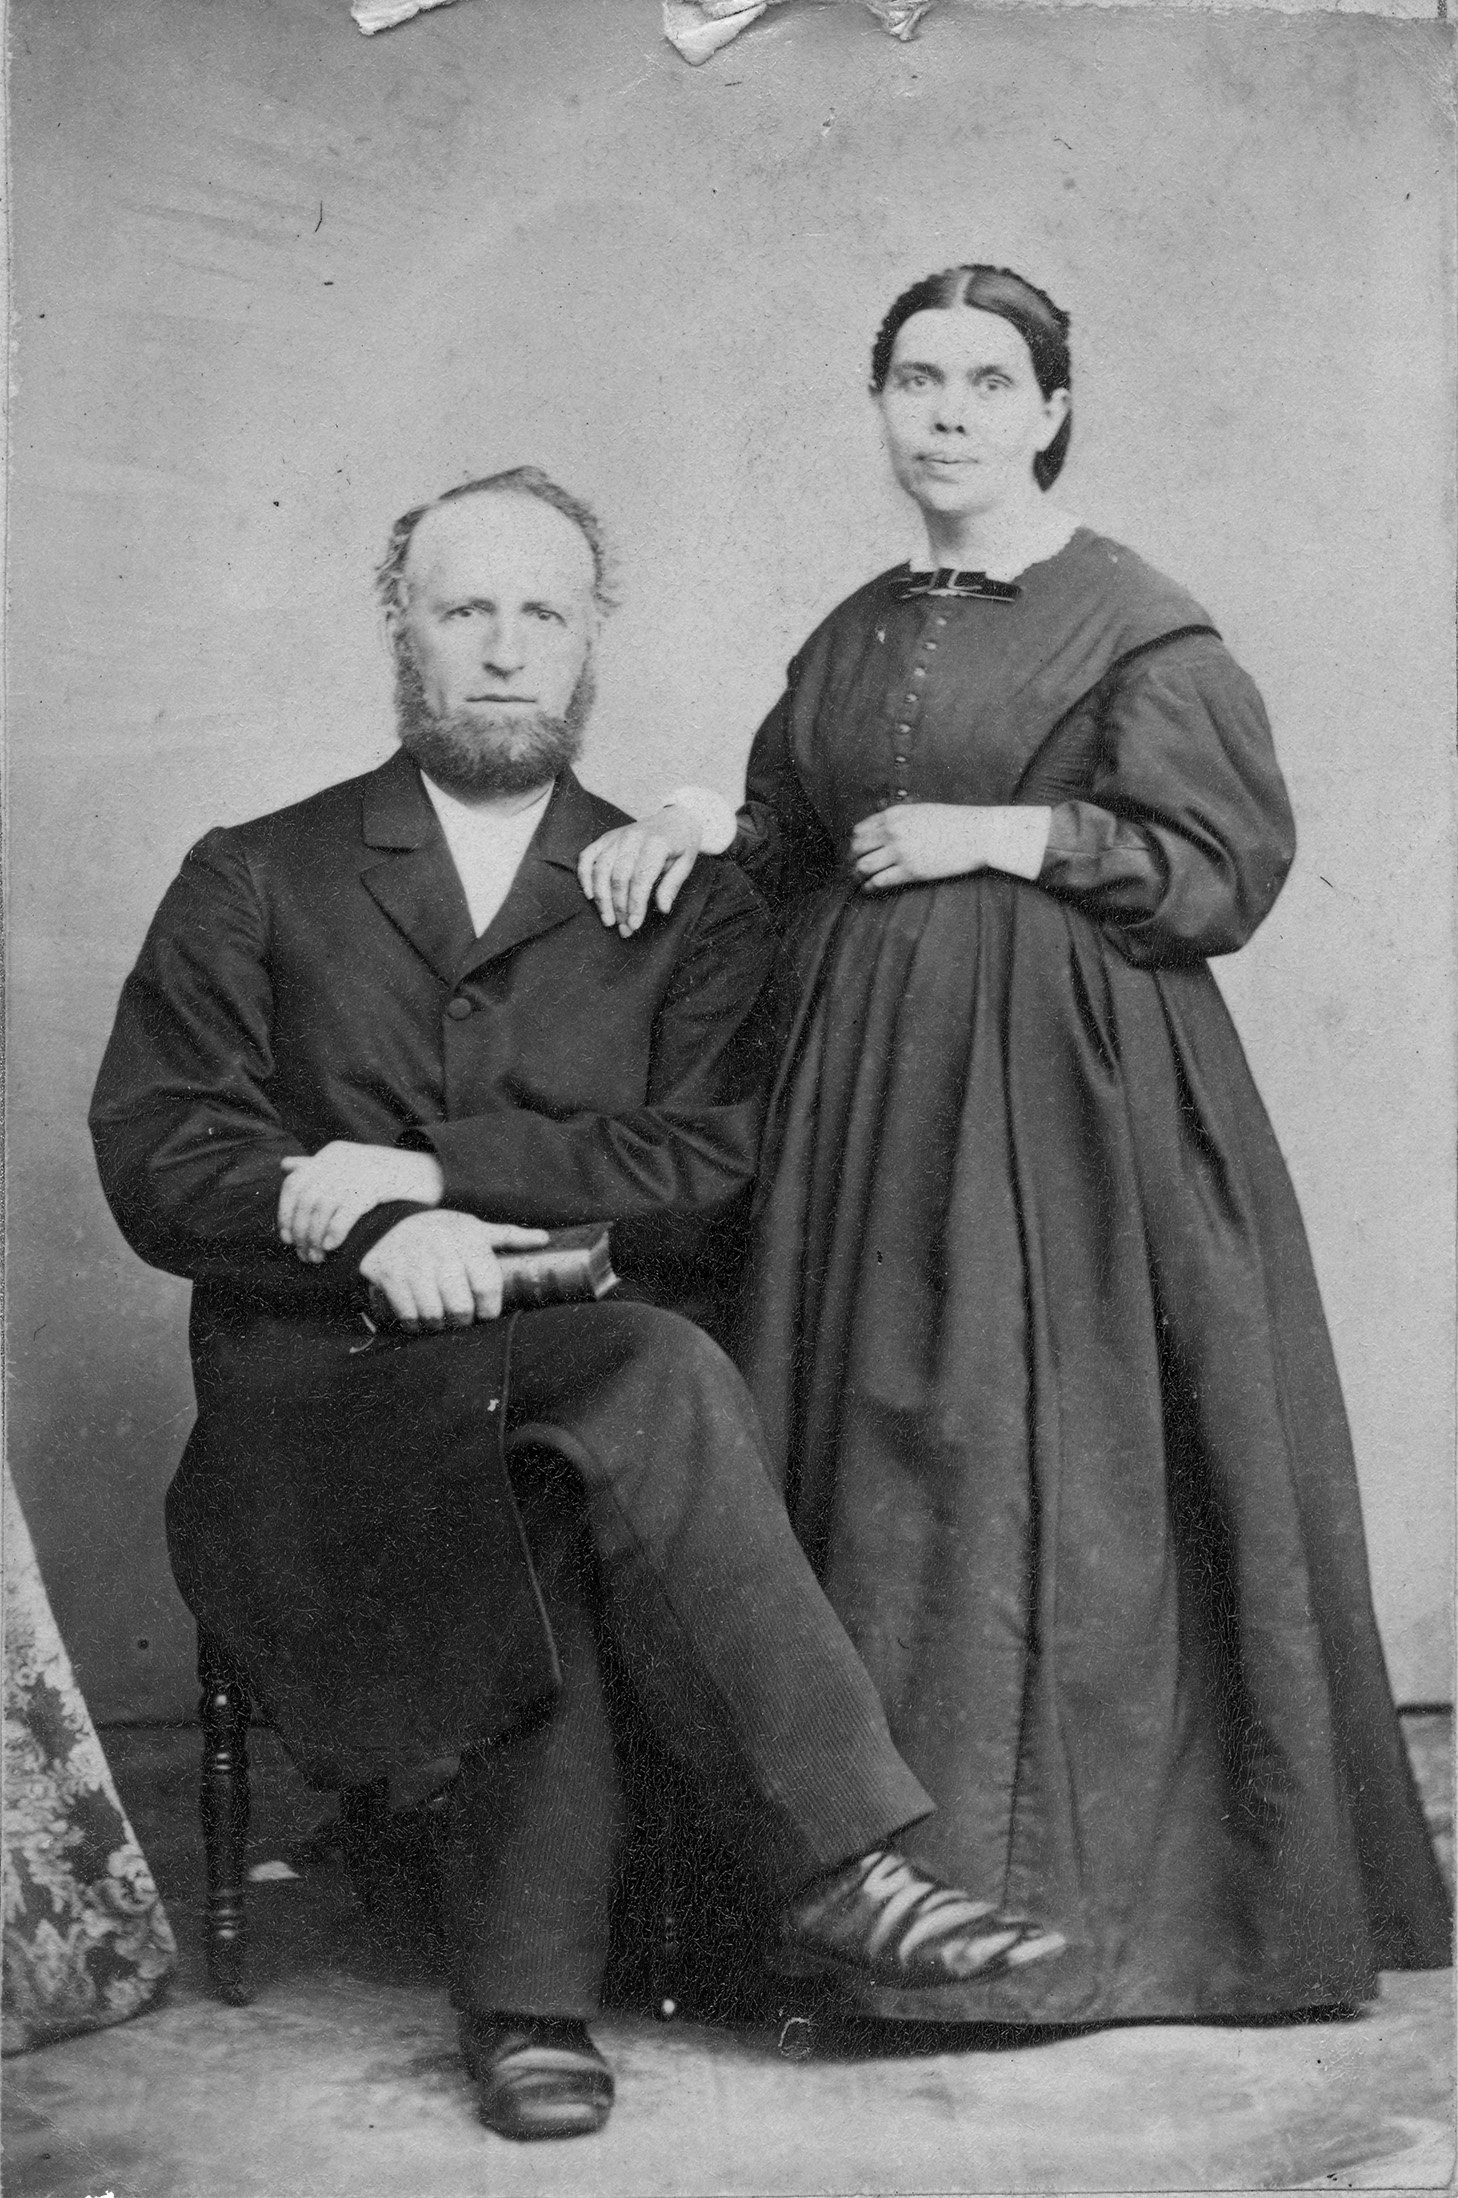
\includegraphics[width=1\linewidth]{images/james-and-ellen-white.jpg}
    \caption*{James Springer White (1821-1881) i Ellen White (1827-1915)}
    \label{fig:james-and-ellen-white}
\end{figure}

\othersQuote{\textbf{ČOVJEK je stvoren na sliku Božju}. ‘I reče Bog: Stvorimo čovjeka na našu sliku, nama sličnoga’. ‘Tako Bog stvori čovjeka na svoju sliku, na sliku Božju stvori ga.’ Postanak 1:26, 27. Vidi također poglavlje. 9:6; 1. Korinćanima 11:7. \textbf{Oni koji poriču ličnost Boga, kažu da ‘slika’ ovdje ne znači \underline{fizički oblik}, već moralnu sliku, i to čine glavnom polaznom točkom za dokazivanje besmrtnosti svih ljudi}. Argument ide ovako: Prvo, čovjek je stvoren na Božju moralnu sliku. Drugo, Bog je besmrtno biće. Treće, stoga su svi ljudi besmrtni. Ali ovaj način razmišljanja također bi dokazao da je čovjek svemoćan, sveznajući i sveprisutan, i tako obukao smrtnog čovjeka u sve atribute božanstva. Pokušajmo: Prvo, čovjek je stvoren na Božju moralnu sliku. Drugo, Bog je svemoguć, sveznajući i sveprisutan. Treće, dakle, čovjek je svemoguć, sveznajući i sveprisutan. Ono što dokazuje previše, ne dokazuje ništa, stoga se stajalište da Božja slika znači njegovu moralnu sliku ne može održati. \textbf{Kao dokaz da je Bog osoba, pročitajte njegove riječi Mojsiju}: ‘I reče Gospod: »Evo mjesta uza me, a ti stani na stijenu. I dogodit će se, dok moja slava bude prolazila, da ću te staviti u raspuklinu stijene i \textbf{svojom te rukom} zakloniti dok \textbf{ne prođem}. Onda ću \textbf{ruku svoju} maknuti, pa ćeš me \textbf{vidjeti odostrag}; \textbf{ali se lice moje ne može vidjeti}.’ Izlazak 33:21-23. Vidi također poglavlje. 24:9-11. \textbf{Ovdje Bog govori Mojsiju da će \underline{vidjeti njegov oblik}}. \textbf{Reći da je Bog učinio da se Mojsiju čini kako vidi njegov oblik, kada on nema oblik, znači optužiti Boga da je uz neistinu dodao i neku vrstu mađioničarske obmane svom sluzi Mojsiju}.}[James S. White, PERGO 1.1; 1861][https://egwwritings.org/read?panels=p1471.3]

\othersQuoteNoGap{No skeptik misli da vidi proturječje između 11. stiha, koji kaže da je Gospod govorio Mojsiju licem u lice, i 20. stiha, koji kaže da Mojsije nije mogao vidjeti njegovo lice. Ali neka Brojevi 12:5-8 otklone poteškoće. ‘\textbf{Tada Gospod siđe u stupu od oblaka}, te stane na ulaz u Šator i zovne Arona i Mirjam. I njih dvoje istupiše. Onda reče: Počujte sad riječi moje: Nađe li se prorok među vama, ja, Gospod, u viđenju se njemu javljam, u snu njemu progovaram. Nije tako sa slugom mojim Mojsijem, on je vjeran u svemu domu mojemu. \textbf{Ustima u usta njemu progovaram, i to \underline{jasno}}.’}[James S. White, PERGO 2.1; 1861][https://egwwritings.org/read?panels=p1471.6]

\othersQuoteNoGap{Veliki i strašni Bog je sišao, obavijen oblakom slave. \textbf{Taj se oblak mogao vidjeti, ali ne i lice koje ima blistaviju svjetlinu od tisuću sunaca}. Pod tim okolnostima, Mojsiju je bilo dopušteno da se približi i \textbf{razgovara s Bogom licem u lice, ili usta na usta, čak i \underline{naizgled}}.}[James S. White, PERGO 2.2; 1861][https://egwwritings.org/read?panels=p1471.7]

\othersQuoteNoGap{Prorok Daniel kaže: ‘Gledao sam sve dok prijestolja ne bijahu zbačena i \textbf{Drevnik vjekova ne sjede}, odjeća mu bijaše bijela kao snijeg, \textbf{a kosa na glavi njegovoj kao čista vuna}; \textbf{prijestolje mu kao plamenovi ognjeni, a kotači mu kao rasplamsali oganj}.’ Poglavlje 7:9. ‘Gledah u noćnim viđenjima, i gle, netko nalik Sinu Čovječjemu dolažaše s oblacima nebeskim i \textbf{dospije do Drevnika vjekova}, i \textbf{dovedoše ga preda nj}, i njemu bȋ predana vlast i slava i kraljevstvo.’ Stihovi 13, 14.}[James S. White, PERGO 2.3; 1861][https://egwwritings.org/read?panels=p1471.8]

\othersQuoteNoGap{Ovdje je uzvišen opis djelovanja \textbf{dviju osoba}; naime, \textbf{Boga Oca i njegovog Sina Isusa Krista}. \textbf{Poreknete li njihove ličnosti, više nemate jasan smisao u ovim citatima iz Daniela}. U vezi s ovim citatom pročitajte izjavu apostola da je \textbf{Sin bio savršena slika osobe svog Oca}. ‘Mnogo puta i na mnogo načina Bog negda progovori ocima po prorocima, a u ovim posljednjim danima progovori nama po Sinu, kojega postavi baštinikom svega, po kojemu i sazda svjetove; \textbf{on, koji je odsjaj slave i savršena slika njegove osobe}.’ Hebrejima 1:1-3.}[James S. White, PERGO 3.1; 1861][https://egwwritings.org/read?panels=p1471.11]

\othersQuoteNoGap{Mi ovdje dodajemo Kristovo svjedočanstvo. ‘I sam Otac, koji me posla, svjedoči za mene. Niti ste čuli njegov glas ikada \textbf{niti ste vidjeli njegov oblik}.’ Ivan 5:37. Vidi i Filipljanima 2:6. \textbf{Reći da Otac nema osobni oblik, čini se da je najizraženija kontradikcija jednostavnih izraza iz Svetih pisama}. \\
PRIGOVOR. - ‘\textbf{\underline{Bog je Duh}}.’ Ivan 4:24.}[James S. White, PERGO 3.2; 1861][https://egwwritings.org/read?panels=p1471.12]

\othersQuoteNoGap{ODGOVOR. - \textbf{Anđeli su također duhovi} [Psalam 104:4], ipak oni koji su posjetili Abrama i Lota, legli su, jeli i uhvatili Lotovu ruku. \textbf{Oni su duhovna bića. Tako je i Bog duhovno biće}.}[James S. White, PERGO 3.3; 1861][https://egwwritings.org/read?panels=p1471.13]

\othersQuoteNoGap{PRIGOVOR. - \textbf{Bog je posvuda}. Dokaz. Psalam 139:1-8. \textbf{On je jednako na svakom mjestu kao da je na jednom mjestu}.}[James S. White, PERGO 3.4; 1861][https://egwwritings.org/read?panels=p1471.14]

\othersQuoteNoGap{ODG. - 1. \textbf{Bog je svugdje na temelju svoga sveznanja}, kao što će se vidjeti iz samih riječi Davida. Stihovi 1-6. ‘O Gospode, \textbf{proničeš me i poznaješ}. \textbf{Ti znaš} kada sjednem i kada ustanem, \textbf{prozireš} namisao moju izdaleka. Moju stazu i lijeganje moje ispituješ, i svi moji putovi \textbf{tebi su znani}. Riječ mi još nije na jeziku, kad gle, Gospode, \textbf{svu je znadeš}. Straga i sprijeda ti me obuhvaćaš, i ruku svoju na mene stavljaš. \textbf{Ta spoznaja} odveć mi je čudesna, previsoka je, dokučit’ je ne mogu.’}[James S. White, PERGO 3.5; 1861][https://egwwritings.org/read?panels=p1471.15]

\othersQuoteNoGap{2. \textbf{Bog je \underline{svugdje prisutan svojstvom svoga Duha}, \underline{koji je njegov predstavnik}, i očituje se gdje god mu se svidi}, kao što će se vidjeti na samim riječima koje prigovarač navodi, a koje se spominje gore. Stihovi 7-10. ‘\textbf{Kamo da odem od \underline{Duha tvojega}}? \textbf{i kamo da od \underline{prisutnosti tvoje} pobjegnem}? Ako se popnem na nebo, ti si ondje; ako si u Šeolu prostrem, evo tebe. Uzmem li krila zorina, nastanim li se nakraj mora, i ondje bi me ruka tvoja vodila, i držala me desnica tvoja.’}[James S. White, PERGO 4.1; 1861][https://egwwritings.org/read?panels=p1471.18]

\othersQuoteNoGap{\textbf{Bog je na nebu}. To smo učeni u Gospodinovoj molitvi. ‘\textbf{Oče naš koji jesi na nebesima}’. Matej 6:9; Luka 11:2. \textbf{Ali ako je Bog jednako na svakom mjestu kao da je na jednom mjestu, onda je nebo isto toliko na svakom mjestu kao da je na jednom mjestu, i ideja o odlasku na nebo je zabluda}. Svi smo na nebu; i Gospodinova molitva, prema ovoj maglovitoj teologiji jednostavno znači, Oče naš \textbf{koji jesi svugdje}, sveti se ime tvoje. Dođi kraljevstvo tvoje; budi volja tvoja kako na zemlji, \textbf{tako i svugdje}.}[James S. White, PERGO 4.2; 1861][https://egwwritings.org/read?panels=p1471.19]

\othersQuoteNoGap{Opet, čitatelji Biblije su vjerovali da su Enoh i Ilija doista bili uzeti \textbf{Bogu na nebo}. \textbf{Ali ako su Bog i nebo jednako na svakom mjestu kao na bilo kojem mjestu, sve je onda to zabluda}. Oni nisu bili uzneseni. I sve što je rečeno o vatrenim kolima i vatrenim konjima, i o vihoru koji je došao da odvede Iliju na nebo, bila je beskorisna parada. Oni su samo isparili, a maglovita para prošla je kroz cijeli svemir. To je sve od Enoha i Ilije što um može shvatiti, \textbf{priznajući da Bog i nebo više nisu na jednom mjestu nego na svakom mjestu}. Ali za Iliju se kaže da je ‘\textbf{uzišao} u vihoru \textbf{u nebo}.’ 2 Kraljevi 2:11. O Henoku se kaže da je ‘hodio s Bogom i nestade, jer ga je Bog uzeo.’ Postanak 5:24.}[James S. White, PERGO 4.3; 1861][https://egwwritings.org/read?panels=p1471.20]

\othersQuoteNoGap{\textbf{Za Isusa se kaže da je s desne strane Veličanstva na visini}. Hebrejima 1:3. ‘Tada Gospodin, nakon što im sve to izgovori, \textbf{bȋ uzet \underline{u nebo}}, \textbf{i sjede zdesna Bogu}.’ Marko 16:19. \textbf{Ali ako je nebo posvuda, i Bog posvuda, onda Kristovo uzašašće na nebo zdesna Ocu, jednostavno znači da je on išao svugdje}! On je bio samo odveden tamo gdje ga je oblak sakrio od pogleda svojih učenika, a zatim ispario i otišao svugdje! Tako da umjesto lijepog Isusa, tako lijepo opisanog u oba Zavjeta, imamo samo neku vrstu bîti raspršene po cijelom svemiru. I u skladu s tom razrijeđenom teologijom, Kristov drugi dolazak, ili njegov povratak, bio bi kondenziranje ove bîti na neki lokalitet, recimo na Maslinsku goru! \textbf{Krist je iz mrtvih ustao u fizičkom obliku}. ‘On nije ovdje’, reče anđeo, ‘jer je uskrsnuo kao što je rekao.’ Matej 28:6.}[James S. White, PERGO 5.1; 1861][https://egwwritings.org/read?panels=p1471.23]

\othersQuoteNoGap{‘I dok su išle javiti njegovim učenicima, gle, dođe im ususret Isus govoreći: »Zdravo!« A one pristupe, \textbf{obujme mu noge}, i poklone mu se.’ Stih 9.}[James S. White, PERGO 5.2; 1861][https://egwwritings.org/read?panels=p1471.24]

\othersQuoteNoGap{‘\textbf{Pogledajte moje ruke i noge},’ reče Isus onima koji su sumnjali u njegovo uskrsnuće, ‘ja sam, glavom! \textbf{Opipajte me i vidite, \underline{duh nema tijela i kostiju} kao što vidite da ja imam}.’ ‘\textbf{I to rekavši, pokaza im ruke i noge}. A dok oni još od radosti nisu vjerovali i čudili se, reče im: »Imate li ovdje što za jelo?« A oni mu dadoše komad pečene ribe i meda u saću. On uzme i pojede pred njima.’ Luka 24:39-43.}[James S. White, PERGO 5.3; 1861][https://egwwritings.org/read?panels=p1471.25]

\othersQuoteNoGap{Nakon što se Isus obratio svojim učenicima na Maslinskoj gori, \textbf{on je bio uzet od njih}, i oblak ga je primio izvan njihovih pogleda. ‘I dok su očiju uprtih \textbf{u nebo gledali kako on odlazi}, gle, stadoše kraj njih dva čovjeka u bijeloj odjeći, koji rekoše: »Ljudi Galilejci, što stojite i gledate u nebo? Ovaj Isus koji je \textbf{od vas uzet u nebo}, isto će tako doći kao što ste ga vidjeli da \textbf{u nebo odlazi}«.’ Djela 1:9-11. J. W.}[James S. White, PERGO 6.1; 1861][https://egwwritings.org/read?panels=p1471.27]

James White se bori protiv ideje da je Bog samo duh, i kao takav, prisutan \others{jednako na svakom mjestu kao na bilo kojem mjestu}. On daje jasno i pozitivno svjedočanstvo iz Pisma da je Bog osobno biće; iste sentimente vidimo u spisima Ellen White.

\egw{Moćna sila koja djeluje kroz čitavu prirodu i održava sve što postoji nije, kao što to prikazuju neki znanstvenici, \textbf{samo jedno sveobuhvatno načelo}, jedna pokretačka energija. \textbf{\underline{Bog jeste duh, a ipak je osobno Biće}}, \textbf{jer je čovjek stvoren po Njegovom obličju}. \textbf{Kao \underline{osobno biće}}, Bog je otkrio Sebe u Svojemu Sinu. Isus, odsjaj Očeve slave, “i \textbf{savršena \underline{slika Njegove osobe}}” (Hebrejima 1:3), našao se na zemlji u obličju čovjeka. Kao \textbf{osobni Spasitelj} On je došao na svijet. Kao \textbf{osobni Spasitelj On je uzašao \underline{na visinu}}. Kao \textbf{osobni Spasitelj On posreduje \underline{u nebeskim dvorima}}. \textbf{Pred prijestoljem Božjim} u naše ime služi ‘Nalik Sinu Čovječjemu.’ Daniel 7:13.}[Ed 131.5; 1903][https://egwwritings.org/read?panels=p29.632]

Ellen White i pioniri adventizma napravili su razliku između pojmova ‘\textit{duh}’ i ‘\textit{biće}’. Bog je osobno biće, a ne samo duh. On nije \others{jednako na svakom mjestu kao na bilo kojem mjestu}, nego je\others{na jednom mjestu više nego na drugom}[John. N. Loughborough, “\textit{Is God a Person?}” The Adventist Review and Sabbath Herald, 18. rujna 1855][https://documents.adventistarchives.org/Periodicals/RH/RH18550918-V07-06.pdf]. On je na nebu, u svom hramu, sjedi na svom prijestolju—osobno—i svuda je prisutan preko svog predstavnika, Svetog Duha.

Evo nekoliko drugih citata sestre White koji su u skladu s pogledima pionira po pitanju \emcap{ličnosti Boga}:

\egw{On \normaltext{[Isus]} je učio da je Bog onaj koji nagrađuje pravedne i kažnjava prijestupnike. \textbf{On nije bio neopipljivi duh}, već živi vladar svemira. \textbf{Ovaj milostivi Otac} je neprestano radio za dobro čovjeka i bio je svjestan svega što se njega tiče...}[3SP 47.1; 1878][https://egwwritings.org/read?panels=p142.195]

\egw{\textbf{Biblija nam pokazuje \underline{Boga na Njegovom uzvišenom i svetom mjestu}}, ne u stanju neaktivnosti, ne u tišini i samoći, već okruženog deset tisuća puta deset tisuća i tisuće tisuća svetih bića, koji svi čekaju izvršiti Njegovu volju. \textbf{Preko ovih glasnika On je u aktivnoj komunikaciji sa svakim dijelom svoje vladavine}. \textbf{\underline{Svojim Duhom On je svugdje prisutan}}. \textbf{Kroz djelovanje svog Duha i svojih anđela} On služi djeci ljudskoj.}[MH 417.2; 1905][https://egwwritings.org/read?panels=p135.2136]

\egw{Veličina Božja je za nas neshvatljiva. ‘\textbf{GOSPOD je u svom svetom Hramu}’ (Psalam 11:4); \textbf{\underline{ipak, po svom Duhu je svuda prisutan}}. \textbf{Ima intimno znanje} o, i osobni interes za, sva djela Svoje ruke.}[Ed 132.2; 1903][https://egwwritings.org/read?panels=p29.636]

\egw{Kroz Isusa Krista, \textbf{Bog—ne parfem, \underline{ne nešto neopipljivo}, \underline{već osobni Bog}}—stvorio je čovjeka i obdario ga inteligencijom i moći.}[Ms117-1898.10; 1898][https://egwwritings.org/read?panels=p7182.15]

Nastavljajući s pamfletom Jamesa Whitea, čitamo njegovu oštru kritiku na razumijevanje Boga kao nematerijalnog. Prije toga, kratko se prisjetimo Dr. Kelloggovog argumenta da\others{\textbf{\underline{Rasprave o Božjem obliku su krajnje besmislene}}}[Dr. John H. Kellogg, The Living Temple, str. 33.][https://archive.org/details/J.H.Kellogg.TheLivingTemple1903/page/n33/] jer je Bog\others{\textbf{daleko izvan našeg shvaćanja \underline{kao što su granice prostora i vremena}}}. Vjerovao je da Božja ličnost nije ograničena na jednu lokaciju jer je Bog \others{jednako na svakom mjestu kao na bilo kojem mjestu}[James S. White, PERGO 4.3; 1861][https://egwwritings.org/read?panels=p1471.20] \footnote{U Živom hramu, Dr. Kellogg je prigovorio da Bog ne može biti svuda prisutan odjednom: “\textit{Kaže netko}, ‘Bog može biti prisutan svojim Duhom, ili svojom moći, ali sigurno sam Bog \textit{ne može biti prisutan svuda odjednom}.’ Mi odgovaramo: Kako se moć može odvojiti od izvora moći? Gdje Božji Duh djeluje, gdje se Božja moć očituje, sam Bog je \textit{stvarno i istinski prisutan}…“ \href{https://archive.org/details/J.H.Kellogg.TheLivingTemple1903/page/n29/}{John H. Kellogg, The Living Temple, str. 28}.}. Ako bi Bog u svojoj ličnosti doista bilo konkretno biće, imajući opipljivo tijelo, tada ne bi mogao biti prisutan \others{jednako na svakom mjestu kao na bilo kojem mjestu} i time održavati život. James White nastavlja protiv razmišljanja da je Bog nematerijalan u svojoj ličnosti.

\othersQuote{NEMATERIJALNOST}

\othersQuoteNoGap{\textbf{OVO je samo drugo ime za ništavnost}. \textbf{To je negacija svih} \textbf{stvari i} \textbf{\underline{bića}} - svega što postoji. Ne postoji ni jedan djelić dokaza koji bi potvrdio njegovo postojanje. Nema načina da se manifestira bilo kojoj inteligenciji na nebu ili na zemlji. \textbf{Ni Bog, ni anđeli, ni ljudi ne bi mogli pojmiti takvu supstancu, biće ili stvar}. \textbf{Ne posjeduje nijedno svojstvo ili moć kojom bi \underline{se moglo manifestirati bilo kojem inteligentnom biću} u svemiru}. Razum i analogija ga nikad ne mogu sagledati, pa čak ni zamisliti. \textbf{Otkrivenje ga nikad ne otkriva, niti ijedno od naših osjetila svjedoči o njegovom postojanju}. \textbf{Ne može se vidjeti, osjetiti, čuti, okusiti ili namirisati, čak ni najjačim organima ili najosjetljivijim osjetilima}. Nije ni tekuće ni kruto, ni meko ni tvrdo - ne može se ni širiti ni skupljati. Ukratko, ne može vršiti nikakav utjecaj - ne može ni djelovati niti se na njega može djelovati. I čak i ako postoji, ne može biti ni od kakve koristi. Ne posjeduje nijedno poželjno svojstvo, sposobnost ili upotrebu, pa ipak, čudno je reći, \textbf{nematerijalnost je moderni kršćanski Bog}, \textbf{njegovo očekivano nebo}, \textbf{njegovo besmrtno ja} - \textbf{njegov sve}!}[James S. White, PERGO 6.2; 1861][https://egwwritings.org/read?panels=p1471.29]


\othersQuoteNoGap{\textbf{O sektaštvo! O ateizam!! O uništenje!!!} \textbf{tko može uočiti fine nijanse razlike između jednog i drugog?} Čine se jednakima, osim po imenu. \textbf{Ateist nema Boga. \underline{Sektaš ima Boga bez tijela ili dijelova}.} Tko može definirati razliku? Što se nas tiče, ne vidimo razliku ni za dlaku; \textbf{oboje tvrde da su negacija svih stvari koje postoje} - i oboje su jednako nemoćni i nepoznati.}[James S. White, PERGO 6.3; 1861][https://egwwritings.org/read?panels=p1471.30]

\othersQuoteNoGap{\textbf{Ateist nema života nakon smrti ili svjesno postojanje nakon groba. Sektaš ima jedan, \underline{ali je nematerijalan, poput njegovog Boga; i bez tijela ili dijelova}. I ovdje su oboje negativni i oboje dolaze do iste točke}. Njihova vjera i nada iznose isto; samo je izraženo različitim pojmovima.}[James S. White, PERGO 7.1; 1861][https://egwwritings.org/read?panels=p1471.33]

\othersQuoteNoGap{Nadalje, \textbf{ateist nema nebo u vječnosti}. \textbf{Sektaš ima jedno, ali je \underline{nematerijalno u svim svojim svojstvima}, i stoga je negacija svog bogatstva i supstanci}. I ovdje su jednaki i dolaze do iste točke.}[James S. White, PERGO 7.2; 1861][https://egwwritings.org/read?panels=p1471.34]

\othersQuoteNoGap{Budući da im ne zavidimo na posjedovanju svega što tvrde, sada ćemo ih ostaviti u mirnom i neometanom uživanju istog, i nastaviti ispitivati dio koji je još uvijek preostao prezrenom materijalistu da uživa.}[James S. White, PERGO 7.3; 1861][https://egwwritings.org/read?panels=p1471.35]

\othersQuoteNoGap{\textbf{Što je Bog? On je materijalna, organizirana inteligencija, \underline{koja posjeduje i tijelo i dijelove}. Čovjek je stvoren na njegovu sliku.}}[James S. White, PERGO 7.4; 1861][https://egwwritings.org/read?panels=p1471.36]

\othersQuoteNoGap{\textbf{Što je Isus Krist? On je Sin Božji, i \underline{sličan je svome Ocu}, budući da je ‘sjaj slave svoga Oca i savršena slika njegove osobe.’ \underline{On je materijalna inteligencija, s tijelom, dijelovima} i čežnjama; koji posjeduje besmrtno tijelo i besmrtne kosti}.}[James S. White, PERGO 7.5; 1861][https://egwwritings.org/read?panels=p1471.37]

\othersQuoteNoGap{\textbf{Što su ljudi?} Oni su Adamovo potomstvo. \textbf{Sposobni su primiti inteligenciju i uzvišenje do takvog stupnja da budu \underline{uskrsnuti od mrtvih s tijelom poput onoga Isusa Krista}, \underline{i posjedovati besmrtno meso i kosti}}. Tako usavršeni, posjedovat će \textbf{materijalni svemir}, to jest zemlju, kao svoje ‘vječno nasljedstvo.’ S ovim nadama i izgledima pred nama, kažemo kršćanskom svijetu koji se drži nematerijalnosti, da su dobrodošli svome Bogu - svom životu - svom nebu i svemu svome. Oni ne traže ništa osim onoga što mi odbacujemo; a mi ne tražimo ništa osim onoga što oni odbacuju. \textbf{Stoga nema razloga za svađu ili sukob među nama}.}[James S. White, PERGO 7.6; 1861][https://egwwritings.org/read?panels=p1471.38]

\othersQuoteNoGap{Mi biramo stvarnost, opipljivu i jasnu, \\
Dok sektaš nestvarnost drži kao spasnu; \\
Svatko nek' uživa što sam odabere, \\
Bez zavisti, u miru, svatko svoje pobere. \\
Nematerijalni Bog njihova je vjera, \\
Za takvog Boga nemamo mi mjera; \\
\textbf{Nematerijalno nebo njihov je dom,} \\
\textbf{U takvom mjestu ne živimo mi tom.} \\
\textbf{Zemlja i nebo naše je pravo,} \\
\textbf{I zvjezdano prostranstvo što sjaji zdravo;} \\
\textbf{Zlato i srebro, dragulji bez broja,} \\
\textbf{I tijela od mesa, to je vjera moja.} \\
\textbf{Takva je nada kad izbavi nas Bog,} \\
\textbf{Od pada Adamovog i grijeha tog;} \\
\textbf{Sve stvari bit će vječno nam dane,} \\
\textbf{Gospodnji ćemo biti sve rajske dane.}}[James S. White, PERGO 8.1; 1861][https://egwwritings.org/read?panels=p1471.41]\footnote{Navedene poezija je prilagođena izvornom tekstu. Poezija u originalu: \\ \others{We choose all substance - what remains \\
The mystical sectarian gains; \\
All that each claims, each shall possess, \\
Nor grudge each other’s happiness. \\
An immaterial God they choose, \\
For such a God we have no use; \\
\textbf{An immaterial heaven and hell,} \\
\textbf{In such a heaven we cannot dwell.} \\
\textbf{We claim the earth, the air, and sky,} \\
\textbf{And all the starry worlds on high;} \\
\textbf{Gold, silver, ore, and precious stones,} \\
\textbf{And bodies made of flesh and bones.} \\
\textbf{Such is our hope, our heaven, our all,} \\
\textbf{When once redeemed from Adam’s fall;} \\
\textbf{All things are ours, and we shall be,} \\
\textbf{The Lord’s to all eternity}.}}

James White uspoređuje sentimente o nematerijalnom Bogu s sektaštvom, ateizmom i uništenjem. “Nematerijalni Bog” je drugi izraz za ništavnost Boga. James White nikada nije primio nikakvu kritiku od sestre White glede njegovih pogleda; naprotiv, već su bila podržana njezinim pisanjem. Mnogi tvrde da je sestra White s vremenom promijenila svoja gledišta i kasnije prihvatila doktrinu o Trojstvu, ali to nije potkrijepljeno detaljnim povijesnim činjenicama. Godine 1905., sestra White prisjeća se događaja s Dr. Kelloggom kada je, dvadeset godina prije, došao k njoj s upravo tim sentimentima o \emcap{ličnosti Boga} koje su James White i drugi pioniri pobijali:

\egw{Dakle, ova tema je preda mnom već više od dvadeset godina. Moj suprug je preminuo prije dvadeset godina, i prije nego što je umro, pojavile su se stvari. Dr. Kellogg je ušao u moju sobu; zauzimala sam jednu od velikih soba u uredu kao svoj dom. Imala sam dvije ili tri sobe tamo, i \textbf{on je dobio veliko svjetlo}; i sjeo je i rekao kakvo je njegovo svjetlo: \textbf{to su iste teorije ili zablude, iste sofisterije, koje on predstavlja, i koje je predstavio u ‘Živom Hramu.’} Rekla sam, ‘Dr. Kellogg, \textbf{ja sam se s tim već susrela.}’ Susrela sam se s tim kad sam prvi put krenula putovati. Susrela sam se s tim na Sjeveru; susrela sam se s tim u New Hampshireu. Vidjela sam prokletstvo njegovog utjecaja u Massachusettsu, i \textbf{svjedočanstva koja su mi dana bila su izravna o tome da ne smijemo imati ništa slično tome što bi se učilo u našim crkvama}. I razgovarala sam s njim. \textbf{Ispričala sam povijest}—nemam vremena da vam je ovdje ispričam. \textbf{Ispričala sam mu povijest o tome kako je to tretirao Božji Duh, i kako mi kao narod moramo izbjeći sofisterije i zablude}. A bili su to propovjednici koji su zavaravali ljude tim sofisterijama. \textbf{Neću vam reći do čega su dovele}—\textbf{možda će to morati doći}; ali neću vam sada reći do čega su dovele; \textbf{ali reći ću vam do čega ove sofisterije vode:} \textbf{One vode do \underline{ništavnosti Krista, do ništavnosti Boga}, \underline{Njegove ličnosti}, i uvode,—kako da to nazovem?—neku vrstu \underline{proizvedene teorije o Bogu i Kristu}}.}[Ms70a-1905.11; 1905][https://egwwritings.org/read?panels=p12696.17]

Kelloggovi sentimenti u “Živom hramu” o \emcap{ličnosti Boga} vode do ništavnosti Krista i ništavnosti Boga. Zašto? Jer njegovi pogledi na Boga tvrde da je Bog nematerijalan. Crkva se suočila s takvim sentimentima na početku svog djelovanja. James White pisao je o njima u svom pamfletu “\textit{Ličnost Boga}”, a sestra White prisjećala se tih ranih iskustava kada su ona i njezin muž borili se protiv zablude da je Bog nematerijalni, sveprisutni duh.

% The personality of God by James White

